\section{Dictionary construction and model census}\label{app:dict}
For GPT-2 small at layer 6 the dictionary holds $50{,}257$ token embedding rows and $1{,}024$ position embedding rows, and for each of blocks 0 to 6 it holds $3{,}072$ MLP down-projection rows, a 64-vector SVD basis of the output-projection row space of each of the 12 attention heads, which amounts to 768 attention atoms per block, and the attention and MLP output biases. The total is $m = 78{,}175$ atoms, about 102 times overcomplete in $d = 768$. Each atom is unit-normed and carries the label of its block, its component and its write subspace. For the other families we take the same census at the middle layer $L$, with the down-projection columns as MLP write directions where the projection is a standard linear layer and no bias atoms. The family sweep restricts embedding atoms to the tokens of the evaluation slice; the attribution rerun keeps each embedding row, which is why its dictionaries are larger. Table~\ref{app:census} lists the models.
\begin{table}[H]\centering\small
\caption{The eight models: width, MLP width, depth, dictionary layer, dictionary sizes and clean cross-entropy on the evaluation tokens (32{,}768 for GPT-2 small, 8{,}192 for the sweep). The 7B-class rows were run in bfloat16.}\label{app:census}
\begin{adjustbox}{max width=\linewidth}
\begin{tabular}{lrrrrrrr}\toprule
Model & $d$ & $d_{\mathrm{ff}}$ & blocks & $L$ & atoms, sweep & atoms, attribution & clean CE \\ \midrule
GPT-2 small & 768 & 3072 & 12 & 6 & 78,175 & 78,175 & 3.647 \\
SmolLM2-135M & 576 & 1536 & 30 & 15 & 36,545 & 82,944 & 3.079 \\
Qwen2.5-0.5B & 896 & 4864 & 24 & 12 & 77,661 & 226,816 & 2.853 \\
Pythia-410m & 1024 & 4096 & 24 & 12 & 69,580 & 116,864 & 3.113 \\
OLMo-1B & 2048 & 8192 & 16 & 8 & 95,180 & 142,464 & 2.570 \\
Qwen2.5-7B & 3584 & 18944 & 28 & 14 & 340,701 & 489,984 & 2.053 \\
Llama-7B & 4096 & 11008 & 32 & 16 & 259,434 & 288,768 & 2.100 \\
Pythia-6.9B & 4096 & 16384 & 32 & 16 & 351,180 & 398,592 & 2.564 \\
\bottomrule\end{tabular}\end{adjustbox}
\end{table}
\section{Reconstruction}\label{app:recon}
The tables of this section are over all states; Appendix~\ref{app:z-gpt2} gives the same sweep and controls over the typical states, and Section~\ref{sec:setup} defines the split. Table~\ref{app:fvu} gives the full sparsity sweep together with the effect of splicing each reconstruction back into the forward pass, and Table~\ref{app:prov} the three provenance controls. The uncentered weight dictionary is the same dictionary applied to raw rather than mean-centered states.
\begin{table}[H]\centering\footnotesize
\caption{Reconstruction of GPT-2 layer-6 states over all 32{,}768 tokens, sink states included: fraction of variance unexplained at each sparsity, and the change in cross-entropy and the KL divergence to the clean next-token distribution when the reconstruction replaces the state in the forward pass. Clean cross-entropy is 3.647.}\label{app:fvu}
\begin{adjustbox}{max width=\linewidth}
\begin{tabular}{lrrrrrrrrrr}\toprule
Dictionary & atoms & FVU $k{=}4$ & 8 & 16 & 32 & 64 & $\Delta$CE 32 & $\Delta$CE 64 & KL 32 & KL 64 \\ \midrule
random directions & 78,175 & 0.911 & 0.833 & 0.700 & 0.501 & 0.252 & +4.613 & +2.690 & 4.546 & 2.623 \\
PCA basis &  & 0.157 & 0.138 & 0.118 & 0.095 & 0.069 & +1.215 & +0.568 & 1.307 & 0.647 \\
weight dictionary & 78,175 & 0.144 & 0.122 & 0.098 & 0.069 & 0.036 & +0.551 & +0.178 & 0.519 & 0.159 \\
weight dictionary, uncentered & 78,175 & 0.182 & 0.148 & 0.114 & 0.079 & 0.042 & +0.644 & +0.208 & 0.570 & 0.171 \\
activation dictionary & 78,175 & 0.058 & 0.045 & 0.034 & 0.023 & 0.013 & +0.053 & +0.014 & 0.096 & 0.040 \\
weight dictionary, layer 8 & 85,859 & 0.227 & 0.193 & 0.154 & 0.108 & 0.056 & +0.386 & +0.142 & 0.352 & 0.121 \\
\bottomrule\end{tabular}\end{adjustbox}
\end{table}
\begin{table}[H]\centering\small
\caption{Provenance controls on the same states, over all states. The rotation preserves the Gram matrix of the dictionary and destroys its alignment with the residual coordinates; the future-block dictionary contains only atoms that could not have written to a layer-6 state.}\label{app:prov}
\begin{adjustbox}{max width=\linewidth}
\begin{tabular}{lrrrrrr}\toprule
Dictionary & atoms & FVU $k{=}4$ & 8 & 16 & 32 & 64 \\ \midrule
weight dictionary after one Gram-preserving rotation & 78,175 & 0.924 & 0.855 & 0.737 & 0.549 & 0.299 \\
correct dictionary subsampled to the future-block size & 70,491 & 0.150 & 0.128 & 0.102 & 0.073 & 0.040 \\
blocks 7 to 11 only, embeddings kept & 70,491 & 0.165 & 0.147 & 0.123 & 0.091 & 0.051 \\
\bottomrule\end{tabular}\end{adjustbox}
\end{table}
\section{Attribution and observability}\label{app:attrib}
Table~\ref{app:survbins} is the data behind the right panel of Figure~\ref{fig:fvu}. Table~\ref{app:auc} asks which property of a write predicts whether OMP identifies it; prominence is circular for one-shot ranking, which selects by prominence, so the informative rows are survival and the rest. Tables~\ref{app:oracle} to~\ref{app:probe} are the oracle baselines, the near-duplicate clustering, the causal tracking checks and the information-survival probe cited in Section~\ref{sec:attrib}.
\begin{table}[H]\centering\small
\caption{Top-1 identification rate of each token's three dominant MLP writes (98,304 cases) by the survival of the write in the layer-6 state. Overall rates: OMP 0.491, one-shot 0.639; among intact writes 0.584, among erased writes 0.0079.}\label{app:survbins}
\begin{adjustbox}{max width=\linewidth}
\begin{tabular}{lrrrr}\toprule
Survival bin & writes & share of cases & identified, OMP & identified, one-shot \\ \midrule
$s<0.0$ & 11,312 & 0.115 & 0.007 & 0.104 \\
$0.0\le s<0.25$ & 1,316 & 0.013 & 0.012 & 0.000 \\
$0.25\le s<0.5$ & 1,574 & 0.016 & 0.036 & 0.000 \\
$0.5\le s<0.75$ & 2,164 & 0.022 & 0.114 & 0.003 \\
$0.75\le s<1.25$ & 11,076 & 0.113 & 0.364 & 0.257 \\
$s\ge 1.25$ & 70,862 & 0.721 & 0.618 & 0.829 \\
\bottomrule\end{tabular}\end{adjustbox}
\end{table}
\begin{table}[H]\centering\small
\caption{Area under the ROC curve for predicting whether OMP identifies a dominant write, one property at a time. Survival and prominence predict; write age does not.}\label{app:auc}
\begin{adjustbox}{max width=\linewidth}
\begin{tabular}{lr}\toprule
Predictor & AUC for OMP identification \\ \midrule
survival $(\mathbf{x}\cdot\mathbf{d})/c$ & 0.733 \\
prominence $|\mathbf{x}\cdot\mathbf{d}|/\lVert\mathbf{x}\rVert$ & 0.803 \\
magnitude $|c|$ & 0.680 \\
relative magnitude $|c|/\lVert\mathbf{x}\rVert$ & 0.652 \\
write age, $6$ minus the source block & 0.511 \\
competition, max $|\cos|$ with the token's other top-8 write directions & 0.307 \\
\bottomrule\end{tabular}\end{adjustbox}
\end{table}
\begin{table}[H]\centering\small
\caption{Two oracles that locate the identification ceiling. Synthetic states built only from each token's own MLP writes give the same recall as real states, so the ceiling belongs to the writes cancelling each other, not to attention or the embedding. Refitting on the true support alone gives a far worse coefficient correlation than the joint sparse fit.}\label{app:oracle}
\begin{adjustbox}{max width=\linewidth}
\begin{tabular}{lr}\toprule
Oracle baseline (16,384 tokens) & value \\ \midrule
synthetic states, sum of the token's MLP writes only: top-1 recall, OMP & 0.621 \\
\quad top-1 recall, one-shot & 0.670 \\
\quad top-3 recall, OMP & 0.466 \\
\quad $r$ on identified writes & 0.998 \\
real states, same tokens: top-1 recall OMP / one-shot & 0.647 / 0.766 \\
least squares on the true top-3 atoms only: $r$, all dominant writes & 0.555 \\
\quad $r$ on erased writes, survival below 0.25 ($n=1,972$) & 0.128 \\
\quad $r$ on intact writes, survival above 0.75 ($n=46,444$) & 0.555 \\
MLP atom coherence: median / 99th percentile / max of max $|\cos|$ to another atom & 0.245 / 0.841 / 0.996 \\
\bottomrule\end{tabular}\end{adjustbox}
\end{table}
\begin{table}[H]\centering\footnotesize
\caption{Near-duplicate atoms merged into clusters at two cosine thresholds; a hit on any atom of the true write's cluster counts. Atom-level top-1 recall is 0.647, so duplication explains almost none of the misses.}\label{app:clusters}
\begin{adjustbox}{max width=\linewidth}
\begin{tabular}{lrrrrrrr}\toprule
cosine $\tau$ & multi-atom clusters & atoms in them & largest & top-1 OMP & top-1 one-shot & top-3 OMP & $r$ identified \\ \midrule
0.95 & 11 & 1,114 & 1021 & 0.650 & 0.766 & 0.492 & 0.999 \\
0.9 & 58 & 1,242 & 1022 & 0.664 & 0.771 & 0.502 & 0.999 \\
\bottomrule\end{tabular}\end{adjustbox}
\end{table}
\begin{table}[H]\centering\small
\caption{Does the decomposition track causal changes? A known write added to a state is recovered at slope 0.90; changing a real source neuron's activation moves its recovered coefficient at slope 0.64.}\label{app:causal}
\begin{adjustbox}{max width=\linewidth}
\begin{tabular}{lrrr}\toprule
Causal check & $n$ & $r$ & slope \\ \midrule
injected atom, recovered coefficient vs injected (mean leakage onto other atoms 0.0076) & 512 & 0.751 & 0.900 \\
source intervention, change in recovered coefficient vs change in the true write & 512 & 0.682 & 0.640 \\
\bottomrule\end{tabular}\end{adjustbox}
\end{table}
\begin{table}[H]\centering\footnotesize
\caption{Leakage-controlled ridge probe from the layer-6 state back to the writer's activation. The write's own direction is a useless readout for erased writers, the full state is not, so erasure is mostly transformation. The probed group is the block-3 neurons whose writes have the lowest mean survival at the layer-6 readout; averaged over all of their firing tokens that survival is 0.80, 0.83, 0.83, 0.86 after blocks 3 to 6, against 2.36, 2.52, 2.71 for the control group of intact writers from blocks 4 to 6, so the group is defined by low survival relative to the population, not by the erasure of every write.}\label{app:probe}
\begin{adjustbox}{max width=\linewidth}
\begin{tabular}{lrrrrr}\toprule
Writer group & neurons & median out-of-sample $R^2$, full state & median $R^2$, own direction & transformed & lost \\ \midrule
block-3 writes later erased & 32 & 0.404 & -0.025 & 0.44 & 0.22 \\
intact control writes & 32 & 0.589 & 0.005 & 0.53 & 0.16 \\
\bottomrule\end{tabular}\end{adjustbox}
\end{table}
\section{Generality}\label{app:general}
Table~\ref{app:attribmodels} extends Table~\ref{tab:families} with one-shot recall and the unconditional correlation, Table~\ref{app:deciles} and Figure~\ref{app:decilefig} give the magnitude-decile correlations behind the architectural divide, Table~\ref{app:channels} the channel-robust FVU, Table~\ref{app:conc} the concentration of the largest write, and Table~\ref{app:pile} the Pile replication.
\begin{table}[H]\centering\small
\caption{Attribution in the rerun with full-vocabulary dictionaries on 8{,}192 states per model (GPT-2 small from the audit rerun). The unconditional correlation counts misses as zero.}\label{app:attribmodels}
\begin{adjustbox}{max width=\linewidth}
\begin{tabular}{lrrrrr}\toprule
Model & gated MLP & top-1 recall, OMP & top-1 recall, one-shot & $r$ identified & $r$ unconditional \\ \midrule
GPT-2 small & no & 0.647 & 0.766 & 0.998 & 0.648 \\
SmolLM2-135M & yes & 0.673 & 0.679 & 1.000 & 0.927 \\
Qwen2.5-0.5B & yes & 0.458 & 0.605 & 0.994 & 0.556 \\
Pythia-410m & no & 0.470 & 0.580 & 0.978 & 0.450 \\
OLMo-1B & yes & 0.703 & 0.774 & 0.996 & 0.971 \\
Qwen2.5-7B & yes & 0.684 & 0.005 & 0.549 & 0.312 \\
Llama-7B & yes & 0.980 & 0.911 & 0.999 & 0.998 \\
Pythia-6.9B & no & 0.808 & 0.657 & 0.522 & 0.412 \\
\bottomrule\end{tabular}\end{adjustbox}
\end{table}
\begin{table}[H]\centering\footnotesize
\caption{Correlation between recovered and true coefficients within each magnitude decile of the identified writes, decile 1 smallest. Gated-MLP models hold the correlation in each decile; GPT-2 and Pythia carry it only in the top decile.}\label{app:deciles}
\begin{adjustbox}{max width=\linewidth}
\begin{tabular}{lrrrrrrrrrr}\toprule
Model & 1 & 2 & 3 & 4 & 5 & 6 & 7 & 8 & 9 & 10 \\ \midrule
GPT-2 small & 0.05 & 0.04 & 0.03 & 0.00 & 0.06 & 0.02 & 0.02 & 0.13 & 0.24 & 1.00 \\
SmolLM2-135M & 0.94 & 0.92 & 0.94 & 0.94 & 0.94 & 0.93 & 0.94 & 0.94 & 0.94 & 1.00 \\
Qwen2.5-0.5B & 0.94 & 0.93 & 0.91 & 0.92 & 0.92 & 0.91 & 0.91 & 0.89 & 0.93 & 1.00 \\
Pythia-410m & 0.22 & 0.03 & 0.07 & 0.02 & 0.02 & 0.07 & 0.07 & 0.03 & 0.12 & 1.00 \\
OLMo-1B & 0.94 & 0.95 & 0.94 & 0.94 & 0.93 & 0.93 & 0.92 & 0.92 & 0.91 & 1.00 \\
Qwen2.5-7B & 0.94 & 0.95 & 0.94 & 0.94 & 0.94 & 0.93 & 0.93 & 0.93 & 0.93 & 0.68 \\
Llama-7B & 0.98 & 0.98 & 0.98 & 0.98 & 0.98 & 0.98 & 0.98 & 0.98 & 0.99 & 1.00 \\
Pythia-6.9B & 0.20 & -0.01 & 0.06 & 0.09 & 0.08 & 0.09 & 0.05 & 0.11 & 0.14 & 0.59 \\
\bottomrule\end{tabular}\end{adjustbox}
\end{table}
\begin{figure}[H]\centering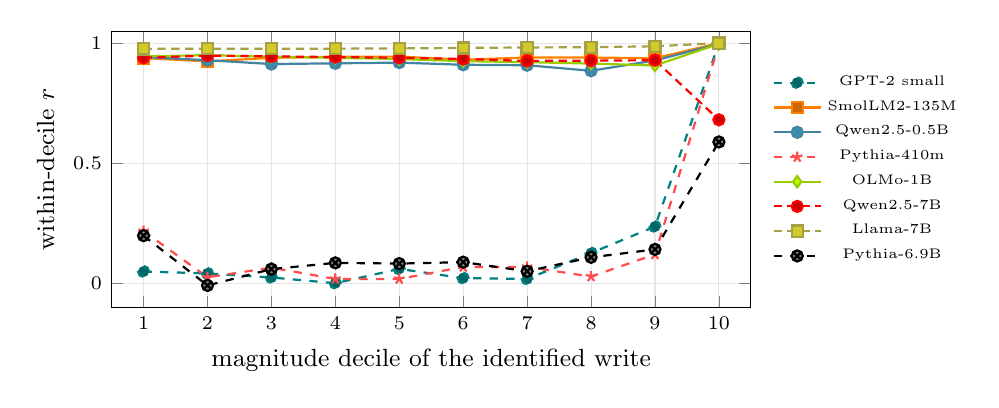
\begin{tikzpicture}\begin{axis}[width=0.8\linewidth, height=0.42\linewidth, xlabel={magnitude decile of the identified write}, ylabel={within-decile $r$}, xmin=0.5, xmax=10.5, ymin=-0.1, ymax=1.05, xtick={1,...,10}, grid=major, grid style={black!10}, legend style={font=\tiny, at={(1.02,0.5)}, anchor=west, draw=none}, tick label style={font=\scriptsize}, label style={font=\small}, cycle list name=exotic]
\addplot+[thick, dashed] coordinates {(1,0.05) (2,0.0421) (3,0.0251) (4,0.0014) (5,0.0608) (6,0.0226) (7,0.019) (8,0.127) (9,0.2371) (10,0.9998)};\addlegendentry{GPT-2 small}
\addplot+[thick] coordinates {(1,0.938) (2,0.924) (3,0.939) (4,0.943) (5,0.944) (6,0.931) (7,0.94) (8,0.94) (9,0.937) (10,1.0)};\addlegendentry{SmolLM2-135M}
\addplot+[thick] coordinates {(1,0.942) (2,0.929) (3,0.913) (4,0.916) (5,0.919) (6,0.91) (7,0.908) (8,0.885) (9,0.928) (10,0.997)};\addlegendentry{Qwen2.5-0.5B}
\addplot+[thick, dashed] coordinates {(1,0.218) (2,0.026) (3,0.066) (4,0.019) (5,0.019) (6,0.069) (7,0.069) (8,0.029) (9,0.121) (10,0.996)};\addlegendentry{Pythia-410m}
\addplot+[thick] coordinates {(1,0.945) (2,0.95) (3,0.943) (4,0.939) (5,0.934) (6,0.925) (7,0.921) (8,0.915) (9,0.907) (10,0.997)};\addlegendentry{OLMo-1B}
\addplot+[thick] coordinates {(1,0.939) (2,0.948) (3,0.945) (4,0.942) (5,0.939) (6,0.934) (7,0.926) (8,0.927) (9,0.929) (10,0.681)};\addlegendentry{Qwen2.5-7B}
\addplot+[thick] coordinates {(1,0.976) (2,0.977) (3,0.977) (4,0.977) (5,0.978) (6,0.98) (7,0.982) (8,0.983) (9,0.987) (10,1.0)};\addlegendentry{Llama-7B}
\addplot+[thick, dashed] coordinates {(1,0.199) (2,-0.008) (3,0.06) (4,0.086) (5,0.083) (6,0.089) (7,0.051) (8,0.109) (9,0.142) (10,0.589)};\addlegendentry{Pythia-6.9B}
\end{axis}\end{tikzpicture}\caption{Within-decile correlation per model. Solid lines are gated-MLP models, dashed lines non-gated.}\label{app:decilefig}\end{figure}
\begin{table}[H]\centering\footnotesize
\caption{The massive-channel test: FVU at $k=32$ over all coordinates and over all but the five highest-variance coordinates, for the weight dictionary and its rotation.}\label{app:channels}
\begin{adjustbox}{max width=\linewidth}
\begin{tabular}{lrrrrr}\toprule
Model & FVU@32, weight & off the top-5 coordinates & FVU@32, rotated & off the top-5 & variance in the top-5 coordinates \\ \midrule
SmolLM2-135M & 0.006 & 0.298 & 0.448 & 13.487 & 98.2\% \\
Qwen2.5-0.5B & 0.017 & 0.350 & 0.518 & 5.367 & 95.2\% \\
Pythia-410m & 0.050 & 0.539 & 0.594 & 3.035 & 91.2\% \\
OLMo-1B & 0.018 & 0.528 & 0.768 & 6.034 & 96.8\% \\
Qwen2.5-7B & 0.010 & 0.226 & 0.851 & 3.728 & 95.8\% \\
Llama-7B & 0.088 & 0.636 & 0.868 & 1.593 & 86.7\% \\
Pythia-6.9B & 0.309 & 0.678 & 0.869 & 1.005 & 55.5\% \\
\bottomrule\end{tabular}\end{adjustbox}
\end{table}
\begin{table}[H]\centering\footnotesize
\caption{Concentration of the largest true write. In all eight models the most frequent top-1 neuron takes a few percent of tokens, so top-1 recall measures identification across thousands of atoms.}\label{app:conc}
\begin{adjustbox}{max width=\linewidth}
\begin{tabular}{lrrrrrr}\toprule
Model & tokens & distinct top-1 neurons & most frequent & which & top five together & entropy, bits \\ \midrule
GPT-2 small & 8,192 & 916 & 4.7\% & mlp0\#132 & 16.5\% & 7.8 \\
SmolLM2-135M & 8,192 & 1,654 & 2.5\% & mlp0\#900 & 10.8\% & 8.9 \\
Qwen2.5-0.5B & 8,192 & 2,275 & 3.4\% & mlp0\#2290 & 9.4\% & 9.7 \\
Pythia-410m & 8,192 & 1,416 & 3.9\% & mlp0\#751 & 11.7\% & 8.9 \\
OLMo-1B & 8,192 & 2,763 & 2.4\% & mlp0\#1913 & 8.9\% & 10.1 \\
Qwen2.5-7B & 8,192 & 3,282 & 3.4\% & mlp9\#11283 & 10.5\% & 10.3 \\
Llama-7B & 8,192 & 2,831 & 4.0\% & mlp16\#4294 & 9.9\% & 10.2 \\
Pythia-6.9B & 8,192 & 1,677 & 8.4\% & mlp14\#2130 & 22.6\% & 8.5 \\
\bottomrule\end{tabular}\end{adjustbox}
\end{table}
\begin{table}[H]\centering\small
\caption{The GPT-2 evaluation on a Pile-derived sample. Reconstruction and attribution replicate; the block-3 role profile does not, which is why the paper treats roles as a property of a model on a distribution. Shuffled-null counter fraction on Pile: 0.668.}\label{app:pile}
\begin{adjustbox}{max width=\linewidth}
\begin{tabular}{lrr}\toprule
GPT-2 small & Pile sample (16,384 tokens) & WikiText-2 \\ \midrule
FVU@32, weight dictionary & 0.080 & 0.069 \\
FVU@32, rotated & 0.518 & 0.520 \\
top-1 recall, OMP & 0.562 & 0.647 \\
top-1 recall, one-shot & 0.660 & 0.766 \\
$r$ identified & 0.998 & 0.998 \\
$r$ unconditional & 0.647 & 0.648 \\
block 3 counter-aligned fraction & 0.379 & 0.525 \\
block 3 median birth survival & 0.77 & -0.09 \\
block 3 anchored fraction & 0.391 & 0.244 \\
\bottomrule\end{tabular}\end{adjustbox}
\end{table}
\begin{figure}[H]\centering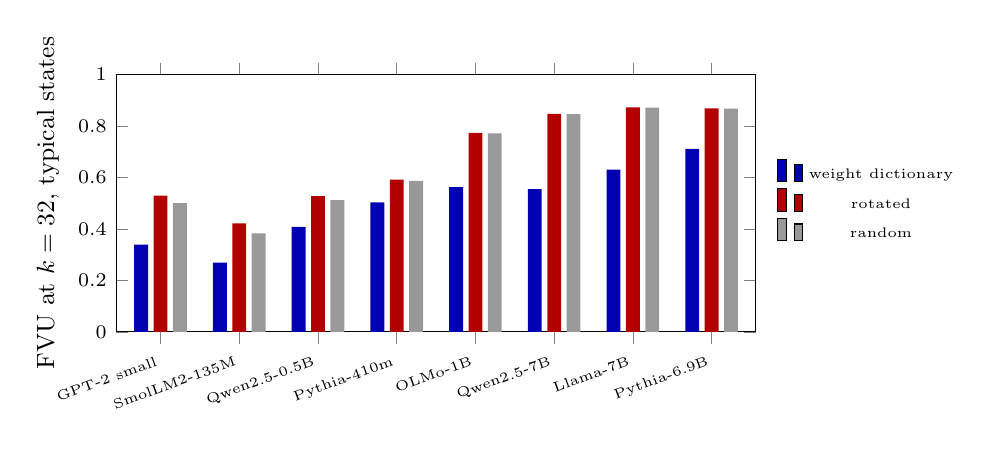
\begin{tikzpicture}\begin{axis}[width=0.8\linewidth, height=0.4\linewidth, ybar, bar width=5pt, ymin=0, ymax=1, ylabel={FVU at $k=32$, typical states}, symbolic x coords={GPT-2 small,SmolLM2-135M,Qwen2.5-0.5B,Pythia-410m,OLMo-1B,Qwen2.5-7B,Llama-7B,Pythia-6.9B}, xtick=data, x tick label style={font=\tiny, rotate=20, anchor=north east}, legend style={font=\tiny, at={(1.02,0.5)}, anchor=west, draw=none}, tick label style={font=\scriptsize}, label style={font=\small}, enlarge x limits=0.08]
\addplot[fill=blue!70!black, draw=none] coordinates {(GPT-2 small,0.3385) (SmolLM2-135M,0.2694) (Qwen2.5-0.5B,0.4076) (Pythia-410m,0.5031) (OLMo-1B,0.5628) (Qwen2.5-7B,0.5548) (Llama-7B,0.6306) (Pythia-6.9B,0.7110)};\addlegendentry{weight dictionary}
\addplot[fill=red!70!black, draw=none] coordinates {(GPT-2 small,0.5294) (SmolLM2-135M,0.4214) (Qwen2.5-0.5B,0.5272) (Pythia-410m,0.5918) (OLMo-1B,0.7731) (Qwen2.5-7B,0.8472) (Llama-7B,0.8723) (Pythia-6.9B,0.8680)};\addlegendentry{rotated}
\addplot[fill=black!40, draw=none] coordinates {(GPT-2 small,0.5002) (SmolLM2-135M,0.3828) (Qwen2.5-0.5B,0.5122) (Pythia-410m,0.5864) (OLMo-1B,0.7709) (Qwen2.5-7B,0.8458) (Llama-7B,0.8717) (Pythia-6.9B,0.8672)};\addlegendentry{random}
\end{axis}\end{tikzpicture}\caption{FVU at $k=32$ per model over the typical states on WikiText-2, from the sweep of Appendix~\ref{app:ci}, for the weight dictionary, its Gram-preserving rotation, and random directions. The rotation sits at the random floor in all eight models.}\label{app:fvufig}\end{figure}
\section{Write roles and null controls}\label{app:roles}
Table~\ref{app:nulls} gives, per block, the real role fractions next to the two nulls, and Table~\ref{app:quint} the counter-aligned fraction by magnitude quintile.
\begin{table}[H]\centering\scriptsize
\caption{Role fractions of each block's dominant writes on WikiText, against random replacement directions and shuffled write-state pairings. Each block's real counter fraction lies below its shuffled null; anchoring and reinforcing mass do not.}\label{app:nulls}
\begin{adjustbox}{max width=\linewidth}
\begin{tabular}{lrrrrrrrrrrr}\toprule
block & writes & median $s_{\mathrm{birth}}$ & counter, real & random dir. & shuffled & anchored, real & random dir. & shuffled & reinforcing, real & random dir. & shuffled \\ \midrule
0 & 39,193 & 1.29 & 0.019 & 0.498 & 0.512 & 0.679 & 0.003 & 0.061 & 0.291 & 0.000 & 0.058 \\
1 & 11,033 & 1.64 & 0.030 & 0.504 & 0.568 & 0.334 & 0.008 & 0.043 & 0.611 & 0.000 & 0.009 \\
2 & 9,989 & 1.02 & 0.197 & 0.495 & 0.637 & 0.403 & 0.012 & 0.064 & 0.335 & 0.000 & 0.021 \\
3 & 10,250 & -0.09 & 0.525 & 0.504 & 0.721 & 0.244 & 0.016 & 0.057 & 0.149 & 0.000 & 0.006 \\
4 & 2,661 & 1.47 & 0.037 & 0.493 & 0.594 & 0.482 & 0.023 & 0.044 & 0.458 & 0.000 & 0.011 \\
5 & 9,556 & 1.54 & 0.237 & 0.508 & 0.633 & 0.201 & 0.040 & 0.067 & 0.524 & 0.000 & 0.014 \\
6 & 15,622 & 1.94 & 0.054 & 0.501 & 0.580 & 0.172 & 0.048 & 0.061 & 0.754 & 0.000 & 0.014 \\
\bottomrule\end{tabular}\end{adjustbox}
\end{table}
\begin{table}[H]\centering\small
\caption{Counter-aligned fraction by magnitude quintile of the write. Block 3 leads in each quintile.}\label{app:quint}
\begin{adjustbox}{max width=\linewidth}
\begin{tabular}{lrrrrr}\toprule
block & quintile 1, smallest & 2 & 3 & 4 & 5, largest \\ \midrule
0 & 0.069 & 0.030 & 0.011 & 0.007 & 0.002 \\
1 & 0.034 & 0.031 & 0.039 & 0.022 & 0.025 \\
2 & 0.270 & 0.213 & 0.203 & 0.170 & 0.097 \\
3 & 0.545 & 0.574 & 0.563 & 0.505 & 0.230 \\
4 & 0.087 & 0.032 & 0.019 & 0.016 & 0.009 \\
5 & 0.378 & 0.315 & 0.177 & 0.044 & 0.012 \\
6 & 0.102 & 0.068 & 0.046 & 0.028 & 0.022 \\
\bottomrule\end{tabular}\end{adjustbox}
\end{table}
\section{The channel-447 circuit}\label{app:circuit}
Tables~\ref{app:dose} to~\ref{app:leash} and Figure~\ref{app:traj} are the intervention results of Section~\ref{sec:circuit} in full.
\begin{table}[H]\centering\footnotesize
\caption{Relative activation change of each active block-3 neuron when channel 447 is scaled at the block 2/3 boundary; 1,236 neurons respond inversely to both scalings by 10\% or more.}\label{app:dose}
\begin{adjustbox}{max width=\linewidth}
\begin{tabular}{lrrrrrrrrr}\toprule
Scaling channel 447 & active neurons & p5 & p25 & median & p75 & p95 & moved 10\% or more & neuron 614 & its percentile \\ \midrule
channel halved & 2948 & +0.2\% & +6.4\% & +9.0\% & +14.0\% & +44.6\% & 45\% & +27.5\% & 90 \\
channel times 1.5 & 2948 & -51.9\% & -17.8\% & -12.0\% & -9.1\% & -5.4\% & 68\% & -21.9\% & 82 \\
\bottomrule\end{tabular}\end{adjustbox}
\end{table}
\begin{table}[H]\centering\footnotesize
\caption{The frozen-normalization control: with block 3's LayerNorm statistics held at their clean-run values, the block-wide response collapses while neuron 614 keeps most of its own.}\label{app:frozen}
\begin{adjustbox}{max width=\linewidth}
\begin{tabular}{lrrrrrrr}\toprule
Block 3 pre-MLP LayerNorm & median, halved & median, times 1.5 & p95, halved & inverse responders & neuron 614, halved & times 1.5 & percentile \\ \midrule
LayerNorm free & +9.0\% & -12.0\% & +44.6\% & 1,236 & +27.5\% & -21.9\% & 90 \\
LayerNorm frozen at clean statistics & -0.5\% & -2.1\% & +17.4\% & 233 & +15.5\% & -12.3\% & 94 \\
\bottomrule\end{tabular}\end{adjustbox}
\end{table}
\begin{table}[H]\centering\small
\caption{Behavioral cost of ablating the strongest channel-447 counter-writers of block 3 (clean cross-entropy 3.6291). The top nine are neurons 614, 2664, 2885, 1995, 2723, 548, 1080, 2600, 2607.}\label{app:ablate}
\begin{adjustbox}{max width=\linewidth}
\begin{tabular}{lrr}\toprule
ablated block-3 counter-writers, top $k$ by counter energy & ablated write energy & $\Delta$CE \\ \midrule
1 & 417,084 & +0.0043 \\
3 & 553,816 & +0.0235 \\
5 & 590,306 & +0.0248 \\
7 & 619,043 & +0.0243 \\
9 & 640,105 & +0.0242 \\
random 9, set 1 & 7,986 & -0.0002 \\
random 9, set 2 & 12,113 & +0.0011 \\
random 9, set 3 & 8,693 & +0.0008 \\
\bottomrule\end{tabular}\end{adjustbox}
\end{table}
\begin{figure}[H]\centering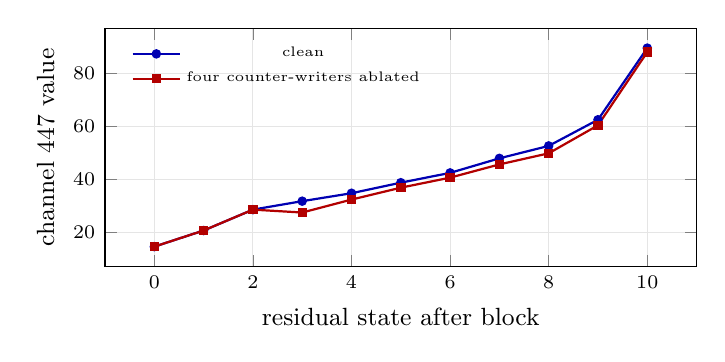
\begin{tikzpicture}\begin{axis}[width=0.75\linewidth, height=0.38\linewidth, xlabel={residual state after block}, ylabel={channel 447 value}, xtick={0,2,...,10}, grid=major, grid style={black!10}, legend style={font=\tiny, at={(0.03,0.97)}, anchor=north west, draw=none, fill=none}, tick label style={font=\scriptsize}, label style={font=\small}]
\addplot[thick, blue!70!black, mark=*, mark size=1.3pt] coordinates {(0,14.6) (1,20.7) (2,28.6) (3,31.8) (4,34.8) (5,38.8) (6,42.5) (7,48.0) (8,52.7) (9,62.6) (10,89.7)};\addlegendentry{clean}
\addplot[thick, red!70!black, mark=square*, mark size=1.3pt] coordinates {(0,14.6) (1,20.7) (2,28.6) (3,27.5) (4,32.4) (5,36.9) (6,40.7) (7,45.7) (8,49.9) (9,60.5) (10,88.2)};\addlegendentry{four counter-writers ablated}
\end{axis}\end{tikzpicture}\caption{Restoration: channel 447 in the raw residual state after each block, with and without the four strongest counter-writers. The ablation opens a gap after block 3 that later components close by the state after block 10, the input of block 11, which is the readout of the text; the state after block 11 is only available through the final normalization and is omitted.}\label{app:traj}\end{figure}
\begin{table}[H]\centering\small
\caption{Per-component contribution to the restoration, summing to -2.22. The largest single restorers are mlp7\#2402 (+1.09), mlp9\#840 (+0.73), mlp10\#900 (+0.64), mlp5\#1888 (+0.53), mlp6\#834 (+0.49).}\label{app:compensate}
\begin{adjustbox}{max width=\linewidth}
\begin{tabular}{lr}\toprule
Component & change in channel 447 write, ablated minus clean \\ \midrule
mlp3 & -4.313 \\
attn4 & +0.340 \\
mlp4 & +1.661 \\
attn5 & +0.755 \\
mlp5 & -0.406 \\
attn6 & +0.226 \\
mlp6 & -0.055 \\
attn7 & -1.863 \\
mlp7 & +1.400 \\
attn8 & -0.535 \\
mlp8 & +0.023 \\
attn9 & -0.570 \\
mlp9 & +1.212 \\
attn10 & -1.415 \\
mlp10 & +2.047 \\
attn11 & +3.127 \\
mlp11 & -3.855 \\
\bottomrule\end{tabular}\end{adjustbox}
\end{table}
\begin{table}[H]\centering\footnotesize
\caption{The reserve bank: channel-insensitive later neurons whose channel-447 writes rise when the four counter-writers are ablated, with random controls for comparison. The primary, neuron 614, is one of the ablated four; its intact write is shown for scale and is zero under the ablation.}\label{app:reserves}
\begin{adjustbox}{max width=\linewidth}
\begin{tabular}{lrrrrrr}\toprule
Neuron & role & gain, halved & gain, times 1.5 & channel-447 write, intact & under group ablation & change \\ \midrule
mlp5\#1888 & reserve & -0.032 & +0.049 & 2.00 & 2.53 & +26\% \\
mlp6\#834 & reserve & -0.030 & +0.031 & 1.84 & 2.33 & +26\% \\
mlp7\#2402 & reserve & -0.031 & +0.063 & 2.13 & 3.23 & +51\% \\
mlp9\#840 & reserve & -0.008 & +0.007 & 7.20 & 7.93 & +10\% \\
mlp10\#900 & reserve & -0.011 & +0.023 & 6.20 & 6.84 & +10\% \\
mlp3\#614 & primary & +0.275 & -0.221 & 4.31 & ablated &  \\
mlp5\#1159 & control & +0.004 & -0.005 & 0.01 & 0.01 & -10\% \\
mlp6\#902 & control & -0.005 & +0.009 & 0.04 & 0.04 & -2\% \\
mlp7\#327 & control & +0.002 & -0.010 & -0.09 & -0.08 & -2\% \\
mlp9\#2312 & control & +0.001 & -0.004 & 0.00 & 0.00 & +0\% \\
mlp10\#2632 & control & +0.012 & -0.014 & -0.03 & -0.03 & +0\% \\
\bottomrule\end{tabular}\end{adjustbox}
\end{table}
\begin{table}[H]\centering\small
\caption{Locating the suppression: which part of the counter-writers' output holds the reserve bank back (clean channel 447 at layer 11: 89.7).}\label{app:leash}
\begin{adjustbox}{max width=\linewidth}
\begin{tabular}{lrrr}\toprule
Write-editing condition & channel 447 at layer 11 & mean reserve response & mean control response \\ \midrule
ablate the four counter-writers & 88.2 & +0.248 & -0.010 \\
remove only the non-channel components of their writes & 91.5 & +0.186 & -0.016 \\
remove only the channel-447 component & 87.0 & +0.046 & +0.007 \\
remove neuron 614's non-channel component alone & 89.6 & -0.002 & +0.000 \\
\bottomrule\end{tabular}\end{adjustbox}
\end{table}
\section{Nomination comparisons}\label{app:bakeoff}
\paragraph{Pre-registered battery.} Fixed in code before any result existed, and identical for each arm. Universe: GPT-2 small MLP neurons in blocks 2 to 8, excluding each neuron studied in the circuit work and any neuron with more than 0.15 of its direction energy in the known massive channels 138, 266, 447, 481 and 496. For a nominee $j$: (1) firing tokens are those with $|c_j|$ in the neuron\textquotesingle s own top 5\%, at least 200; (2) the ledger names the top upstream MLP contributor $u$ along $\mathbf{d}_j$ on those tokens; (3) $u$ is ablated, and as a matched control a random neuron from $u$\textquotesingle s block, measuring on the firing tokens the change in $\langle \mathbf{h}, \mathbf{d}_j\rangle$ after block $j$ against the prediction from $u$\textquotesingle s direct contribution, and the relative change in $|a_j|$; (4) Tier 1 holds when the sign matches the prediction, the magnitude lies within 0.2 to 2 times the prediction, and exceeds 3 times the control; Tier 2 holds when the relative response is at least 0.02 and at least 3 times the control. Arms: WDD ranks by unconditional counter-alignment write energy; the outlier arm by activation excess kurtosis times mean write magnitude; the correlation arm, added at ten per arm, by maximum absolute activation correlation with any upstream MLP neuron.
\begin{table}[H]\centering\footnotesize
\caption{The pilot at three nominees per arm. Fisher exact, one-sided: Tier 2, $p=0.05$; passing either tier, $p=0.20$.}\label{app:pilot}
\begin{adjustbox}{max width=\linewidth}
\begin{tabular}{lrrrrrrrr}\toprule
Nominee & partner $u$ & predicted & measured & control & response & control & Tier 1 & Tier 2 \\ \midrule
\multicolumn{9}{l}{\emph{WDD arm}} \\
mlp6\#437 & mlp5\#1790 & -2.91 & +0.81 & -0.01 & +0.238 & -0.000 & no & yes \\
mlp8\#583 & mlp2\#676 & +3.74 & +9.86 & -0.01 & -0.924 & +0.001 & no & yes \\
mlp2\#1195 & mlp0\#1121 & +1.08 & +0.20 & +0.01 & -0.200 & -0.001 & no & yes \\
\multicolumn{9}{l}{\emph{outlier arm}} \\
mlp8\#1807 & mlp2\#666 & +2.87 & +0.43 & -0.00 & +0.002 & -0.000 & no & no \\
mlp6\#861 & mlp3\#614 & +0.17 & -0.01 & -0.01 & -0.005 & -0.001 & no & no \\
mlp8\#2535 & mlp7\#2367 & -0.32 & -0.23 & +0.00 & +0.017 & +0.001 & yes & no \\
\bottomrule\end{tabular}\end{adjustbox}
\end{table}
\begin{table}[H]\centering\small
\caption{Tallies at ten and thirty nominees per arm. One-sided Fisher exact tests at thirty per arm: WDD against the outlier screen, Tier 2 $p=0.004$ and Tier 1 $p=0.15$; the correlation screen against WDD, Tier 2 $p=0.37$ and Tier 1 $p=0.0017$. The first ten nominees of each thirty-nominee arm are the ten-nominee arms, and their tallies reproduce exactly.}\label{app:tallies}
\begin{adjustbox}{max width=\linewidth}
\begin{tabular}{lrrrr}\toprule
Arm & Tier 1 & Tier 2 & either & both \\ \midrule
\multicolumn{5}{l}{\emph{ten nominees per arm}} \\
WDD & 4/10 & 8/10 & 8/10 & 4/10 \\
outlier & 2/10 & 6/10 & 7/10 & 1/10 \\
corr & 9/10 & 8/10 & 10/10 & 7/10 \\
\multicolumn{5}{l}{\emph{thirty nominees per arm}} \\
WDD & 16/30 & 23/30 & 27/30 & 12/30 \\
outlier & 11/30 & 12/30 & 22/30 & 1/30 \\
corr & 27/30 & 25/30 & 30/30 & 22/30 \\
\bottomrule\end{tabular}\end{adjustbox}
\end{table}
\begin{figure}[H]\centering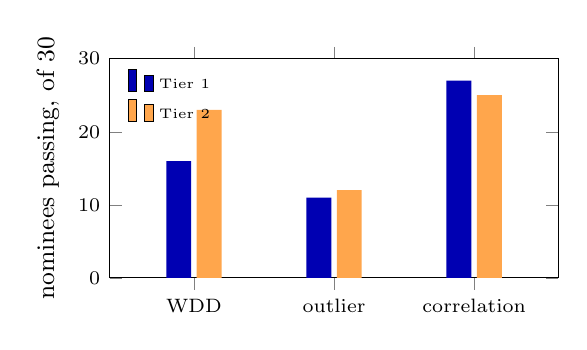
\begin{tikzpicture}\begin{axis}[width=0.6\linewidth, height=0.36\linewidth, ybar, bar width=9pt, ymin=0, ymax=30, ylabel={nominees passing, of 30}, symbolic x coords={WDD,outlier,correlation}, xtick=data, legend style={font=\tiny, at={(0.02,0.98)}, anchor=north west, draw=none, fill=none}, tick label style={font=\scriptsize}, label style={font=\small}, enlarge x limits=0.3]
\addplot[fill=blue!70!black, draw=none] coordinates {(WDD,16) (outlier,11) (correlation,27)};\addlegendentry{Tier 1}
\addplot[fill=orange!70, draw=none] coordinates {(WDD,23) (outlier,12) (correlation,25)};\addlegendentry{Tier 2}
\end{axis}\end{tikzpicture}\caption{The thirty-per-arm bake-off.}\label{app:bakefig}\end{figure}
\begin{center}\scriptsize
\begin{longtable}{llrrrrrcc}
\caption{Each nominee of the thirty-per-arm run, with the arm or arms that nominated it and its battery. Columns as in Table~\ref{app:pilot}.}\label{app:n30}\\ \toprule
Nominee & arms & partner & predicted & measured & control & response & control & T1/T2 \\ \midrule \endfirsthead
\toprule Nominee & arms & partner & predicted & measured & control & response & control & T1/T2 \\ \midrule \endhead
\bottomrule \endfoot
mlp2\#34 & correlation & mlp0\#1561 & -1.87 & -2.17 & -0.03 & -0.282 & -0.002 & yes/yes \\
mlp2\#352 & correlation & mlp1\#3020 & -1.52 & -2.12 & +0.00 & -0.780 & +0.000 & yes/yes \\
mlp2\#589 & WDD & mlp0\#1430 & +0.23 & -0.00 & +0.00 & -0.003 & -0.000 & no/no \\
mlp2\#1173 & outlier, correlation & mlp0\#944 & +0.75 & +0.41 & -0.00 & -0.001 & -0.000 & yes/no \\
mlp2\#1279 & correlation & mlp0\#2009 & +0.78 & -0.24 & -0.01 & +0.062 & +0.001 & no/yes \\
mlp2\#2769 & WDD, correlation & mlp0\#1175 & +5.99 & +8.33 & +0.01 & -0.977 & +0.001 & yes/yes \\
mlp2\#2830 & correlation & mlp0\#1175 & -6.34 & -9.71 & +0.00 & -0.946 & +0.000 & yes/yes \\
mlp2\#2898 & correlation & mlp0\#371 & -0.45 & -0.53 & -0.00 & -0.000 & -0.000 & yes/no \\
mlp3\#176 & WDD & mlp1\#79 & +0.93 & +0.57 & -0.00 & -0.223 & -0.003 & yes/yes \\
mlp3\#489 & outlier & mlp2\#2714 & -0.65 & +0.30 & +0.01 & +0.033 & +0.001 & no/yes \\
mlp4\#825 & correlation & mlp2\#666 & +8.87 & +3.08 & +0.00 & +0.073 & +0.001 & yes/yes \\
mlp4\#1322 & WDD & mlp3\#614 & -1.36 & -0.08 & -0.01 & +0.069 & -0.001 & no/yes \\
mlp4\#2266 & correlation & mlp0\#1451 & -1.09 & -1.58 & +0.01 & -0.367 & -0.002 & yes/yes \\
mlp4\#2555 & correlation & mlp2\#666 & +6.77 & +2.26 & +0.00 & +0.005 & +0.001 & yes/no \\
mlp4\#2806 & correlation & mlp0\#2054 & -4.25 & -7.03 & -0.03 & -0.457 & -0.002 & yes/yes \\
mlp5\#464 & correlation & mlp4\#2622 & -2.05 & -4.26 & -0.01 & -0.531 & -0.002 & no/yes \\
mlp5\#1504 & correlation & mlp0\#132 & -7.66 & -7.42 & -0.00 & -0.251 & +0.001 & yes/yes \\
mlp5\#1526 & outlier & mlp3\#2664 & -0.21 & +0.13 & +0.01 & -0.026 & +0.001 & no/yes \\
mlp5\#2073 & correlation & mlp3\#2614 & -4.31 & -1.06 & -0.00 & -0.258 & -0.000 & yes/yes \\
mlp5\#2078 & outlier & mlp3\#614 & -0.72 & +0.03 & -0.00 & -0.028 & +0.001 & no/yes \\
mlp5\#2084 & correlation & mlp2\#666 & -7.49 & -1.81 & -0.00 & -0.008 & +0.003 & yes/no \\
mlp5\#2256 & outlier, correlation & mlp2\#666 & +10.51 & +2.75 & -0.00 & +0.034 & -0.000 & yes/yes \\
mlp6\#203 & correlation & mlp2\#2830 & -6.54 & -11.85 & -0.01 & -0.920 & -0.003 & yes/yes \\
mlp6\#522 & WDD & mlp4\#1727 & -0.71 & -0.31 & +0.00 & +0.070 & +0.001 & yes/yes \\
mlp6\#1393 & correlation & mlp0\#874 & -2.06 & -1.65 & -0.01 & -0.167 & -0.000 & yes/yes \\
mlp6\#1681 & outlier & mlp2\#2714 & +0.16 & -0.01 & -0.00 & -0.005 & +0.000 & no/no \\
mlp6\#1912 & correlation & mlp0\#908 & -3.59 & -1.33 & -0.02 & -0.053 & -0.001 & yes/yes \\
mlp6\#1985 & WDD & mlp5\#1856 & -0.57 & +0.25 & -0.00 & +0.323 & +0.000 & no/yes \\
mlp6\#2006 & outlier & mlp3\#614 & +0.32 & +0.02 & +0.00 & -0.015 & +0.000 & no/no \\
mlp6\#2081 & correlation & mlp2\#666 & -3.21 & -0.77 & -0.00 & +0.001 & -0.001 & yes/no \\
mlp6\#2374 & correlation & mlp0\#1218 & -1.83 & -1.63 & +0.01 & -0.064 & +0.000 & yes/yes \\
mlp6\#2667 & correlation & mlp0\#753 & -1.21 & -1.96 & +0.00 & -0.315 & -0.000 & yes/yes \\
mlp6\#2674 & WDD & mlp2\#2830 & +5.93 & +10.26 & -0.00 & -0.920 & +0.003 & yes/yes \\
mlp6\#2703 & correlation & mlp0\#132 & -7.57 & -7.46 & +0.01 & -0.249 & -0.000 & yes/yes \\
mlp6\#2984 & outlier & mlp5\#1888 & -0.19 & -0.09 & +0.00 & +0.005 & +0.000 & yes/no \\
mlp6\#3048 & WDD & mlp5\#1790 & -2.05 & +0.24 & +0.00 & +0.222 & +0.000 & no/yes \\
mlp7\#6 & outlier & mlp5\#1790 & +0.51 & +0.15 & -0.01 & -0.013 & -0.000 & yes/no \\
mlp7\#549 & correlation & mlp0\#132 & -6.32 & -5.84 & -0.00 & -0.173 & -0.000 & yes/yes \\
mlp7\#658 & correlation & mlp0\#2963 & -1.29 & -2.42 & -0.01 & -0.294 & -0.001 & yes/yes \\
mlp7\#889 & outlier & mlp3\#614 & +0.59 & +0.13 & -0.01 & +0.013 & -0.001 & yes/no \\
mlp7\#991 & WDD & mlp1\#1825 & -0.37 & -0.22 & -0.00 & -0.427 & -0.003 & yes/yes \\
mlp7\#1600 & WDD & mlp5\#1790 & -0.42 & -0.13 & -0.00 & +0.005 & +0.001 & yes/no \\
mlp7\#1729 & WDD & mlp6\#3039 & +0.60 & -0.04 & +0.00 & +0.033 & +0.000 & no/yes \\
mlp7\#2083 & WDD & mlp6\#2799 & -0.70 & -0.91 & +0.00 & +0.292 & +0.001 & yes/yes \\
mlp7\#2202 & correlation & mlp6\#2081 & -0.75 & -1.48 & -0.00 & -0.348 & -0.000 & yes/yes \\
mlp7\#2214 & outlier & mlp3\#614 & -0.38 & -0.05 & -0.00 & -0.011 & +0.001 & no/no \\
mlp7\#2348 & outlier & mlp5\#1790 & -0.26 & +0.10 & +0.01 & -0.035 & +0.001 & no/yes \\
mlp7\#2398 & WDD & mlp3\#1545 & -1.12 & -0.25 & -0.00 & -0.008 & +0.000 & yes/no \\
mlp7\#2489 & WDD & mlp5\#1790 & -2.05 & +0.40 & -0.00 & -0.072 & +0.001 & no/yes \\
mlp7\#2517 & WDD & mlp6\#1879 & +0.66 & +0.40 & +0.00 & -0.269 & +0.004 & yes/yes \\
mlp7\#2531 & WDD & mlp2\#2771 & +1.57 & -0.05 & -0.00 & -0.030 & +0.001 & no/yes \\
mlp7\#2750 & outlier & mlp6\#3039 & +0.38 & +0.01 & +0.00 & +0.015 & +0.000 & no/no \\
mlp8\#13 & WDD & mlp7\#2367 & -1.43 & +1.34 & +0.00 & +0.013 & -0.000 & no/no \\
mlp8\#15 & WDD & mlp0\#132 & +1.09 & +0.92 & -0.00 & -0.058 & -0.000 & yes/yes \\
mlp8\#82 & outlier & mlp5\#1790 & +0.53 & +0.29 & +0.00 & +0.004 & +0.000 & yes/no \\
mlp8\#201 & correlation & mlp7\#1588 & -0.55 & -0.73 & -0.01 & -0.143 & -0.001 & yes/yes \\
mlp8\#428 & WDD & mlp7\#2367 & +0.61 & -0.73 & +0.03 & -0.100 & +0.003 & no/yes \\
mlp8\#529 & WDD & mlp7\#2690 & -0.79 & -0.45 & -0.01 & +0.219 & -0.004 & yes/yes \\
mlp8\#599 & WDD & mlp7\#2367 & +0.44 & -0.67 & +0.00 & +0.010 & -0.001 & no/no \\
mlp8\#687 & outlier & mlp7\#2367 & +0.88 & -0.66 & -0.00 & +0.120 & -0.001 & no/yes \\
mlp8\#825 & WDD & mlp7\#1012 & +0.90 & -0.24 & -0.00 & -0.288 & -0.003 & no/yes \\
mlp8\#1108 & outlier & mlp7\#2402 & +0.22 & +0.12 & +0.01 & -0.001 & +0.002 & yes/no \\
mlp8\#1182 & outlier & mlp7\#2367 & +0.30 & +0.61 & +0.01 & +0.010 & +0.002 & no/no \\
mlp8\#1203 & WDD & mlp7\#2402 & +0.44 & +0.28 & -0.02 & +0.011 & +0.001 & yes/no \\
mlp8\#1276 & WDD & mlp7\#2402 & +0.35 & +0.05 & +0.01 & -0.027 & +0.001 & no/yes \\
mlp8\#1332 & WDD & mlp7\#79 & +1.30 & +0.57 & +0.01 & -0.283 & +0.000 & yes/yes \\
mlp8\#1333 & correlation & mlp7\#658 & -1.47 & -1.74 & -0.01 & -0.181 & -0.003 & yes/yes \\
mlp8\#1423 & outlier & mlp7\#2402 & +0.62 & +0.34 & -0.00 & -0.007 & -0.000 & yes/no \\
mlp8\#1542 & WDD & mlp7\#2589 & +0.83 & -0.04 & +0.01 & -0.163 & -0.002 & no/yes \\
mlp8\#1749 & outlier & mlp7\#2367 & -0.28 & +0.53 & -0.01 & +0.078 & -0.002 & no/yes \\
mlp8\#1764 & WDD & mlp7\#2086 & -0.20 & -0.12 & +0.00 & +0.040 & +0.002 & yes/yes \\
mlp8\#1827 & WDD & mlp7\#2402 & -1.35 & -0.64 & +0.00 & +0.065 & +0.001 & yes/yes \\
mlp8\#1864 & WDD & mlp5\#1790 & -0.33 & -0.10 & -0.00 & +0.000 & -0.002 & yes/no \\
mlp8\#1981 & WDD & mlp5\#1790 & -0.45 & +0.20 & +0.04 & -0.030 & +0.005 & no/yes \\
mlp8\#2036 & outlier & mlp7\#2367 & -1.11 & +1.86 & +0.04 & -0.010 & +0.001 & no/no \\
mlp8\#2087 & outlier & mlp7\#2367 & +0.78 & -1.10 & -0.02 & +0.010 & -0.001 & no/no \\
mlp8\#2162 & outlier & mlp7\#2367 & +0.56 & -0.77 & -0.01 & +0.061 & -0.002 & no/yes \\
mlp8\#2346 & outlier & mlp7\#2367 & +1.36 & -1.62 & +0.00 & +0.015 & -0.000 & no/no \\
mlp8\#2387 & outlier & mlp5\#1790 & -0.23 & -0.12 & +0.01 & -0.002 & +0.000 & yes/no \\
mlp8\#2402 & outlier & mlp7\#2402 & +0.21 & +0.10 & -0.00 & -0.010 & -0.000 & yes/no \\
mlp8\#2469 & outlier & mlp7\#2367 & +1.66 & -2.13 & -0.00 & +0.036 & -0.000 & no/yes \\
mlp8\#2532 & outlier & mlp4\#1894 & +0.18 & +0.08 & -0.00 & -0.007 & +0.000 & yes/no \\
mlp8\#2543 & outlier & mlp7\#2367 & +1.08 & -1.11 & +0.00 & +0.039 & +0.000 & no/yes \\
mlp8\#2687 & correlation & mlp6\#2081 & -1.35 & -3.27 & -0.01 & -0.482 & -0.001 & no/yes \\
mlp8\#2793 & outlier & mlp7\#2367 & +1.38 & -1.66 & +0.01 & +0.101 & +0.002 & no/yes \\
mlp8\#2836 & outlier & mlp7\#2367 & -0.29 & +1.08 & -0.01 & +0.280 & -0.006 & no/yes \\
mlp8\#2988 & correlation & mlp7\#2233 & -2.41 & -2.36 & +0.01 & -0.209 & +0.001 & yes/yes \\
\end{longtable}\end{center}
\section{Independent recomputation}\label{app:audit}
\begin{table}[H]\centering\small
\caption{An independent re-implementation of the dictionary, the attribution and the dose response, written from the description in the text with its own hooks, batching and seeds, on the same 32{,}768 tokens. The deterministic quantities agree to the printed precision and the dose response to within 0.2 percentage points; the rotation control draws a fresh random rotation (seed 777), so its value is near but not equal to that of Section~\ref{sec:recon}.}\label{app:audit-table}
\begin{adjustbox}{max width=\linewidth}
\begin{tabular}{lrr}\toprule
Quantity & paper & recomputed \\ \midrule
FVU at $k=32$, weight dictionary & 0.069 & 0.069 \\
FVU at $k=32$, rotated (fresh rotation, seed 777) & 0.549 & 0.517 \\
top-1 recall, OMP & 0.647 & 0.647 \\
$r$ identified & 0.998 & 0.998 \\
$r$ unconditional & 0.648 & 0.648 \\
neuron 614 response, channel halved & +27.5\% & +27.5\% \\
neuron 614 response, channel times 1.5 & -22.1\% & -21.9\% \\
\bottomrule\end{tabular}\end{adjustbox}
\end{table}
\section{Confidence intervals and the second corpus}\label{app:ci}
All numbers here come from \texttt{exp\_z2\_ci}, an implementation of the family sweep written from the description in Sections~\ref{sec:method} and~\ref{sec:setup} independently of the individual experiment scripts, run under one protocol for all eight models: 32{,}768 evaluation states per model and corpus, the same three dictionaries, OMP with $k=64$ read at 32 and 64, one-shot attribution, and a bootstrap over the 64 evaluation sequences with 1{,}000 resamples. Brackets are 95\% percentile intervals. GPT-2 keeps the conventions of Section~\ref{sec:setup} (a disjoint centering slice for reconstruction, the evaluation mean for attribution); the other families center on eight disjoint chunks throughout. Table~\ref{app:ci-old} sets its point estimates beside those of the individual experiment scripts.
\begin{table}[H]\centering\scriptsize
\caption{Reconstruction of the typical states on WikiText-2 with 95\% bootstrap intervals over sequences. Off top-5 removes the five highest-variance coordinates from numerator and denominator.}\label{app:ci-recon-wikitext}
\begin{adjustbox}{max width=\linewidth}
\begin{tabular}{lrrrrrrrr}\toprule
Model & FVU@32 weight & FVU@64 weight & FVU@32 rotated & FVU@64 rotated & FVU@32 random & off top-5, weight & off top-5, rotated & top-5 share \\ \midrule
GPT-2 small & 0.338 [0.337, 0.340] & 0.179 [0.179, 0.180] & 0.529 [0.529, 0.530] & 0.288 & 0.500 [0.500, 0.500] & 0.38 & 0.56 & 82.1\% \\
SmolLM2-135M & 0.269 [0.268, 0.270] & 0.113 [0.113, 0.114] & 0.421 [0.421, 0.422] & 0.179 & 0.383 [0.383, 0.383] & 0.34 & 0.49 & 98.2\% \\
Qwen2.5-0.5B & 0.408 [0.407, 0.408] & 0.219 [0.219, 0.219] & 0.527 [0.527, 0.527] & 0.282 & 0.512 [0.512, 0.512] & 0.44 & 0.55 & 95.4\% \\
Pythia-410m & 0.503 [0.502, 0.504] & 0.303 [0.302, 0.303] & 0.592 [0.592, 0.592] & 0.359 & 0.586 [0.586, 0.587] & 0.54 & 0.62 & 91.3\% \\
OLMo-1B & 0.563 [0.561, 0.564] & 0.435 [0.433, 0.436] & 0.773 [0.773, 0.773] & 0.611 & 0.771 [0.771, 0.771] & 0.60 & 0.79 & 96.7\% \\
Qwen2.5-7B & 0.555 [0.551, 0.558] & 0.459 [0.456, 0.462] & 0.847 [0.847, 0.847] & 0.729 & 0.846 [0.846, 0.846] & 0.68 & 0.88 & 95.8\% \\
Llama-7B & 0.631 [0.628, 0.633] & 0.533 [0.531, 0.535] & 0.872 [0.872, 0.872] & 0.772 & 0.872 [0.872, 0.872] & 0.66 & 0.88 & 86.9\% \\
Pythia-6.9B & 0.711 [0.709, 0.713] & 0.610 [0.609, 0.612] & 0.868 [0.868, 0.868] & 0.764 & 0.867 [0.867, 0.867] & 0.74 & 0.87 & 55.9\% \\
\bottomrule\end{tabular}\end{adjustbox}
\end{table}
\begin{table}[H]\centering\scriptsize
\caption{The sink states on WikiText-2: how many of the 32{,}768 states exceed ten times the median norm, the variance they carry, and their reconstruction. The all-state columns are what an FVU over all states reports.}\label{app:ci-sink-wikitext}
\begin{adjustbox}{max width=\linewidth}
\begin{tabular}{lrrrrrrrr}\toprule
Model & sink states & smallest sink norm over median & share of variance & sink FVU@32 weight & rotated & random & all-state FVU@32 weight & rotated \\ \midrule
GPT-2 small & 64 & 44$\times$ & 79.7\% & 0.0003 [0.0003, 0.0003] & 0.532 & 0.508 & 0.069 & 0.531 \\
SmolLM2-135M & 64 & 155$\times$ & 98.1\% & 0.0005 [0.0005, 0.0005] & 0.421 & 0.390 & 0.006 & 0.421 \\
Qwen2.5-0.5B & 65 & 85$\times$ & 96.2\% & 0.0013 [0.0013, 0.0013] & 0.517 & 0.514 & 0.017 & 0.518 \\
Pythia-410m & 127 & 47$\times$ & 90.8\% & 0.0037 [0.0037, 0.0037] & 0.591 & 0.582 & 0.050 & 0.591 \\
OLMo-1B & 68 & 43$\times$ & 96.8\% & 0.0006 [0.0006, 0.0006] & 0.779 & 0.773 & 0.019 & 0.779 \\
Qwen2.5-7B & 65 & 203$\times$ & 99.0\% & 0.0039 [0.0038, 0.0040] & 0.840 & 0.843 & 0.010 & 0.840 \\
Llama-7B & 131 & 27$\times$ & 86.0\% & 0.0002 [0.0002, 0.0002] & 0.870 & 0.870 & 0.089 & 0.870 \\
Pythia-6.9B & 66 & 21$\times$ & 58.7\% & 0.0270 [0.0269, 0.0272] & 0.873 & 0.866 & 0.310 & 0.871 \\
\bottomrule\end{tabular}\end{adjustbox}
\end{table}
\begin{table}[H]\centering\scriptsize
\caption{Attribution on WikiText-2 with 95\% bootstrap intervals over sequences. The all-state correlations are carried by the few identified writes at the sink states, whose magnitudes dominate the statistic; the typical-state columns exclude them, and Table~\ref{app:ci-calib-wikitext} is the accuracy statement.}\label{app:ci-attrib-wikitext}
\begin{adjustbox}{max width=\linewidth}
\begin{tabular}{lrrrrrrrr}\toprule
Model & gated & top-1 recall, OMP & top-1 recall, one-shot & $r$ identified, all states & typical states & $r$ unconditional, all & typical & identified writes \\ \midrule
GPT-2 small & no & 0.647 [0.637, 0.657] & 0.766 [0.754, 0.776] & 0.998 [0.998, 0.998] & 0.582 & 0.648 [0.648, 0.648] & 0.505 & 48,220 \\
SmolLM2-135M & yes & 0.670 [0.661, 0.680] & 0.682 [0.676, 0.688] & 1.000 [1.000, 1.000] & 0.835 & 0.928 [0.927, 0.928] & 0.494 & 48,543 \\
Qwen2.5-0.5B & yes & 0.459 [0.451, 0.467] & 0.614 [0.604, 0.623] & 0.994 [0.993, 0.994] & 0.819 & 0.551 [0.543, 0.559] & 0.534 & 34,285 \\
Pythia-410m & no & 0.481 [0.472, 0.490] & 0.593 [0.584, 0.601] & 0.980 [0.979, 0.981] & 0.322 & 0.452 [0.446, 0.455] & 0.275 & 35,864 \\
OLMo-1B & yes & 0.693 [0.687, 0.699] & 0.779 [0.775, 0.784] & 0.997 [0.997, 0.998] & 0.907 & 0.971 [0.969, 0.972] & 0.762 & 59,579 \\
Qwen2.5-7B & yes & 0.673 [0.663, 0.685] & 0.004 [0.004, 0.005] & 0.554 [0.506, 0.595] & 0.887 & 0.308 [0.271, 0.343] & 0.742 & 54,625 \\
Llama-7B & yes & 0.981 [0.979, 0.983] & 0.895 [0.881, 0.906] & 0.999 [0.999, 0.999] & 0.982 & 0.998 [0.998, 0.998] & 0.970 & 93,027 \\
Pythia-6.9B & no & 0.787 [0.779, 0.795] & 0.646 [0.639, 0.653] & 0.539 [0.528, 0.551] & 0.645 & 0.424 [0.409, 0.439] & 0.482 & 67,509 \\
\bottomrule\end{tabular}\end{adjustbox}
\end{table}
\begin{table}[H]\centering\scriptsize
\caption{Calibration of the recovered coefficients of identified dominant writes on WikiText-2, typical states. Ratio is recovered over true; a ratio above one is over-estimation.}\label{app:ci-calib-wikitext}
\begin{adjustbox}{max width=\linewidth}
\begin{tabular}{lrrrrrrrrrrr}\toprule
Model & identified writes & negative & sign recovered & median relative error & within 25\% & ratio, decile 1 & 5 & 10 & rel. error, decile 1 & 5 & 10 \\ \midrule
GPT-2 small & 48,156 & 0\% & 99.8\% & 0.44 [0.44, 0.45] & 29.4\% & 1.66 & 1.42 & 1.45 & 0.66 & 0.42 & 0.45 \\
SmolLM2-135M & 48,479 & 50\% & 100.0\% & 0.54 [0.53, 0.54] & 26.0\% & 1.97 & 1.55 & 0.73 & 0.97 & 0.55 & 0.32 \\
Qwen2.5-0.5B & 34,220 & 47\% & 100.0\% & 0.46 [0.45, 0.46] & 26.5\% & 1.58 & 1.34 & 0.43 & 0.58 & 0.45 & 0.57 \\
Pythia-410m & 35,801 & 0\% & 99.9\% & 0.41 [0.40, 0.42] & 34.2\% & 1.75 & 1.43 & 1.04 & 0.75 & 0.43 & 0.27 \\
OLMo-1B & 59,503 & 46\% & 99.7\% & 0.34 [0.34, 0.34] & 35.0\% & 1.06 & 0.76 & 0.51 & 0.25 & 0.32 & 0.49 \\
Qwen2.5-7B & 54,601 & 51\% & 100.0\% & 0.50 [0.50, 0.51] & 17.6\% & 0.97 & 0.52 & 0.29 & 0.25 & 0.48 & 0.71 \\
Llama-7B & 92,755 & 49\% & 100.0\% & 0.25 [0.25, 0.25] & 49.8\% & 1.39 & 1.24 & 1.17 & 0.39 & 0.26 & 0.17 \\
Pythia-6.9B & 67,475 & 0\% & 100.0\% & 1.03 [1.02, 1.04] & 4.4\% & 2.19 & 2.03 & 1.86 & 1.19 & 1.03 & 0.86 \\
\bottomrule\end{tabular}\end{adjustbox}
\end{table}
\begin{table}[H]\centering\scriptsize
\caption{Within-decile correlation of recovered and true coefficients on WikiText-2 (point estimates; intervals in Figure~\ref{app:ci-decilefig-wikitext}). In the gated models about half of the writes are negative, so this signed correlation within a magnitude decile mostly records sign recovery, and Table~\ref{app:ci-calib-wikitext} is the accuracy statement.}\label{app:ci-deciles-wikitext}
\begin{adjustbox}{max width=\linewidth}
\begin{tabular}{lrrrrrrrrrr}\toprule
Model & 1 & 2 & 3 & 4 & 5 & 6 & 7 & 8 & 9 & 10 \\ \midrule
GPT-2 small & 0.05 & 0.04 & 0.03 & 0.00 & 0.06 & 0.02 & 0.02 & 0.13 & 0.24 & 1.00 \\
SmolLM2-135M & 0.94 & 0.92 & 0.94 & 0.95 & 0.94 & 0.93 & 0.94 & 0.94 & 0.93 & 1.00 \\
Qwen2.5-0.5B & 0.94 & 0.93 & 0.91 & 0.91 & 0.91 & 0.92 & 0.90 & 0.88 & 0.94 & 1.00 \\
Pythia-410m & 0.21 & 0.03 & 0.08 & 0.02 & -0.05 & -0.02 & 0.03 & 0.07 & -0.07 & 1.00 \\
OLMo-1B & 0.93 & 0.95 & 0.94 & 0.94 & 0.93 & 0.93 & 0.92 & 0.91 & 0.91 & 1.00 \\
Qwen2.5-7B & 0.94 & 0.95 & 0.94 & 0.94 & 0.94 & 0.94 & 0.94 & 0.94 & 0.94 & 0.70 \\
Llama-7B & 0.97 & 0.98 & 0.98 & 0.98 & 0.98 & 0.98 & 0.98 & 0.98 & 0.99 & 1.00 \\
Pythia-6.9B & 0.22 & 0.02 & 0.04 & 0.04 & 0.05 & 0.07 & 0.04 & 0.08 & 0.12 & 0.66 \\
\bottomrule\end{tabular}\end{adjustbox}
\end{table}
\begin{figure}[H]\centering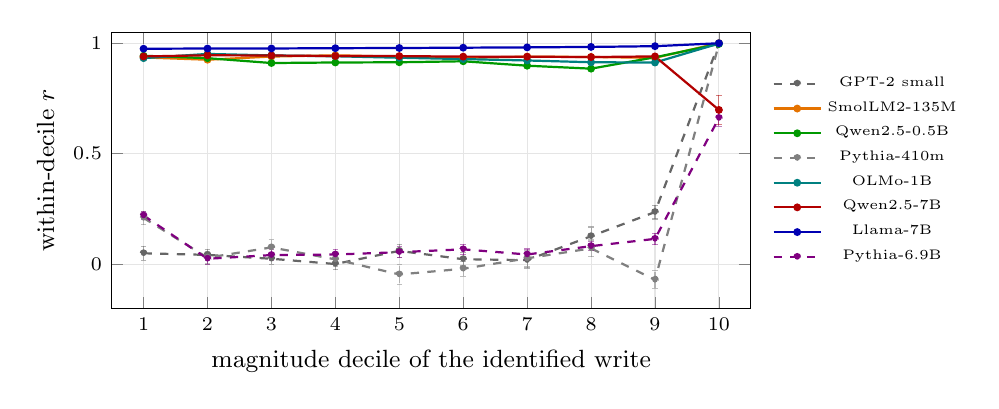
\begin{tikzpicture}\begin{axis}[width=0.8\linewidth, height=0.42\linewidth, xlabel={magnitude decile of the identified write}, ylabel={within-decile $r$}, xmin=0.5, xmax=10.5, ymin=-0.2, ymax=1.05, xtick={1,...,10}, grid=major, grid style={black!10}, legend style={font=\tiny, at={(1.02,0.5)}, anchor=west, draw=none}, tick label style={font=\scriptsize}, label style={font=\small}, error bars/y dir=both, error bars/y explicit]
\addplot[thick, dashed, color=black!60, mark=*, mark size=1pt, error bars/error bar style={opacity=0.5}] coordinates {(1,0.0499) +- (0,0.0322) (2,0.0425) +- (0,0.0256) (3,0.0251) +- (0,0.0254) (4,0.0013) +- (0,0.0260) (5,0.0607) +- (0,0.0294) (6,0.0230) +- (0,0.0301) (7,0.0189) +- (0,0.0354) (8,0.1270) +- (0,0.0416) (9,0.2362) +- (0,0.0312) (10,0.9998) +- (0,0.0000)};\addlegendentry{GPT-2 small}
\addplot[thick, color=orange!90!black, mark=*, mark size=1pt, error bars/error bar style={opacity=0.5}] coordinates {(1,0.9353) +- (0,0.0027) (2,0.9250) +- (0,0.0028) (3,0.9393) +- (0,0.0015) (4,0.9451) +- (0,0.0024) (5,0.9387) +- (0,0.0061) (6,0.9337) +- (0,0.0049) (7,0.9390) +- (0,0.0030) (8,0.9374) +- (0,0.0023) (9,0.9334) +- (0,0.0030) (10,0.9998) +- (0,0.0000)};\addlegendentry{SmolLM2-135M}
\addplot[thick, color=green!60!black, mark=*, mark size=1pt, error bars/error bar style={opacity=0.5}] coordinates {(1,0.9430) +- (0,0.0037) (2,0.9320) +- (0,0.0038) (3,0.9101) +- (0,0.0027) (4,0.9125) +- (0,0.0033) (5,0.9135) +- (0,0.0029) (6,0.9180) +- (0,0.0033) (7,0.8980) +- (0,0.0033) (8,0.8846) +- (0,0.0040) (9,0.9360) +- (0,0.0046) (10,0.9962) +- (0,0.0009)};\addlegendentry{Qwen2.5-0.5B}
\addplot[thick, dashed, color=gray, mark=*, mark size=1pt, error bars/error bar style={opacity=0.5}] coordinates {(1,0.2098) +- (0,0.0308) (2,0.0299) +- (0,0.0286) (3,0.0764) +- (0,0.0343) (4,0.0224) +- (0,0.0321) (5,-0.0458) +- (0,0.0435) (6,-0.0202) +- (0,0.0343) (7,0.0271) +- (0,0.0364) (8,0.0720) +- (0,0.0381) (9,-0.0702) +- (0,0.0402) (10,0.9959) +- (0,0.0004)};\addlegendentry{Pythia-410m}
\addplot[thick, color=teal, mark=*, mark size=1pt, error bars/error bar style={opacity=0.5}] coordinates {(1,0.9322) +- (0,0.0054) (2,0.9512) +- (0,0.0014) (3,0.9445) +- (0,0.0019) (4,0.9406) +- (0,0.0017) (5,0.9340) +- (0,0.0019) (6,0.9279) +- (0,0.0020) (7,0.9216) +- (0,0.0025) (8,0.9136) +- (0,0.0028) (9,0.9123) +- (0,0.0026) (10,0.9982) +- (0,0.0007)};\addlegendentry{OLMo-1B}
\addplot[thick, color=red!70!black, mark=*, mark size=1pt, error bars/error bar style={opacity=0.5}] coordinates {(1,0.9398) +- (0,0.0023) (2,0.9451) +- (0,0.0021) (3,0.9441) +- (0,0.0021) (4,0.9415) +- (0,0.0019) (5,0.9414) +- (0,0.0032) (6,0.9390) +- (0,0.0042) (7,0.9387) +- (0,0.0046) (8,0.9370) +- (0,0.0064) (9,0.9400) +- (0,0.0062) (10,0.6980) +- (0,0.0659)};\addlegendentry{Qwen2.5-7B}
\addplot[thick, color=blue!70!black, mark=*, mark size=1pt, error bars/error bar style={opacity=0.5}] coordinates {(1,0.9747) +- (0,0.0009) (2,0.9756) +- (0,0.0009) (3,0.9759) +- (0,0.0008) (4,0.9771) +- (0,0.0012) (5,0.9780) +- (0,0.0008) (6,0.9794) +- (0,0.0006) (7,0.9808) +- (0,0.0009) (8,0.9829) +- (0,0.0007) (9,0.9862) +- (0,0.0007) (10,0.9995) +- (0,0.0000)};\addlegendentry{Llama-7B}
\addplot[thick, dashed, color=violet, mark=*, mark size=1pt, error bars/error bar style={opacity=0.5}] coordinates {(1,0.2207) +- (0,0.0199) (2,0.0250) +- (0,0.0245) (3,0.0418) +- (0,0.0241) (4,0.0442) +- (0,0.0237) (5,0.0549) +- (0,0.0243) (6,0.0677) +- (0,0.0238) (7,0.0444) +- (0,0.0247) (8,0.0821) +- (0,0.0198) (9,0.1150) +- (0,0.0256) (10,0.6616) +- (0,0.0405)};\addlegendentry{Pythia-6.9B}
\end{axis}\end{tikzpicture}\caption{Within-decile correlation per model on WikiText-2, with 95\% bootstrap intervals as error bars. Solid lines are gated-MLP models, dashed non-gated.}\label{app:ci-decilefig-wikitext}\end{figure}
\begin{table}[H]\centering\scriptsize
\caption{Reconstruction of the typical states on the Pile sample with 95\% bootstrap intervals over sequences. Off top-5 removes the five highest-variance coordinates from numerator and denominator.}\label{app:ci-recon-pile}
\begin{adjustbox}{max width=\linewidth}
\begin{tabular}{lrrrrrrrr}\toprule
Model & FVU@32 weight & FVU@64 weight & FVU@32 rotated & FVU@64 rotated & FVU@32 random & off top-5, weight & off top-5, rotated & top-5 share \\ \midrule
GPT-2 small & 0.358 [0.354, 0.362] & 0.190 [0.188, 0.192] & 0.530 [0.529, 0.530] & 0.288 & 0.500 [0.500, 0.500] & 0.40 & 0.56 & 80.6\% \\
SmolLM2-135M & 0.277 [0.276, 0.279] & 0.117 [0.116, 0.117] & 0.421 [0.421, 0.421] & 0.179 & 0.383 [0.383, 0.383] & 0.35 & 0.49 & 98.2\% \\
Qwen2.5-0.5B & 0.413 [0.411, 0.415] & 0.222 [0.221, 0.223] & 0.528 [0.527, 0.528] & 0.282 & 0.512 [0.512, 0.512] & 0.44 & 0.55 & 95.2\% \\
Pythia-410m & 0.509 [0.507, 0.511] & 0.306 [0.305, 0.307] & 0.592 [0.592, 0.593] & 0.359 & 0.586 [0.586, 0.587] & 0.55 & 0.62 & 91.5\% \\
OLMo-1B & 0.503 [0.502, 0.505] & 0.388 [0.387, 0.389] & 0.773 [0.773, 0.773] & 0.610 & 0.771 [0.771, 0.771] & 0.60 & 0.81 & 98.2\% \\
Qwen2.5-7B & 0.533 [0.530, 0.536] & 0.438 [0.436, 0.440] & 0.847 [0.847, 0.847] & 0.729 & 0.846 [0.846, 0.846] & 0.66 & 0.88 & 95.7\% \\
Llama-7B & 0.627 [0.625, 0.629] & 0.529 [0.527, 0.531] & 0.872 [0.872, 0.872] & 0.772 & 0.872 [0.872, 0.872] & 0.65 & 0.88 & 85.1\% \\
Pythia-6.9B & 0.682 [0.677, 0.688] & 0.584 [0.579, 0.588] & 0.868 [0.868, 0.868] & 0.764 & 0.867 [0.867, 0.867] & 0.72 & 0.88 & 65.5\% \\
\bottomrule\end{tabular}\end{adjustbox}
\end{table}
\begin{table}[H]\centering\scriptsize
\caption{The sink states on the Pile sample: how many of the 32{,}768 states exceed ten times the median norm, the variance they carry, and their reconstruction. The all-state columns are what an FVU over all states reports.}\label{app:ci-sink-pile}
\begin{adjustbox}{max width=\linewidth}
\begin{tabular}{lrrrrrrrr}\toprule
Model & sink states & smallest sink norm over median & share of variance & sink FVU@32 weight & rotated & random & all-state FVU@32 weight & rotated \\ \midrule
GPT-2 small & 64 & 41$\times$ & 77.9\% & 0.0003 [0.0003, 0.0003] & 0.533 & 0.507 & 0.079 & 0.532 \\
SmolLM2-135M & 66 & 158$\times$ & 98.1\% & 0.0005 [0.0005, 0.0005] & 0.421 & 0.390 & 0.006 & 0.421 \\
Qwen2.5-0.5B & 64 & 102$\times$ & 96.0\% & 0.0013 [0.0013, 0.0014] & 0.517 & 0.514 & 0.018 & 0.517 \\
Pythia-410m & 129 & 41$\times$ & 91.2\% & 0.0037 [0.0037, 0.0038] & 0.591 & 0.582 & 0.048 & 0.591 \\
OLMo-1B & 173 & 33$\times$ & 98.4\% & 0.0005 [0.0004, 0.0005] & 0.778 & 0.774 & 0.009 & 0.778 \\
Qwen2.5-7B & 64 & 124$\times$ & 98.9\% & 0.0039 [0.0038, 0.0040] & 0.840 & 0.843 & 0.010 & 0.840 \\
Llama-7B & 132 & 10$\times$ & 84.3\% & 0.0002 [0.0002, 0.0002] & 0.870 & 0.870 & 0.098 & 0.870 \\
Pythia-6.9B & 129 & 10$\times$ & 69.2\% & 0.0269 [0.0268, 0.0270] & 0.873 & 0.866 & 0.229 & 0.872 \\
\bottomrule\end{tabular}\end{adjustbox}
\end{table}
\begin{table}[H]\centering\scriptsize
\caption{Attribution on the Pile sample with 95\% bootstrap intervals over sequences. The all-state correlations are carried by the few identified writes at the sink states, whose magnitudes dominate the statistic; the typical-state columns exclude them, and Table~\ref{app:ci-calib-pile} is the accuracy statement.}\label{app:ci-attrib-pile}
\begin{adjustbox}{max width=\linewidth}
\begin{tabular}{lrrrrrrrr}\toprule
Model & gated & top-1 recall, OMP & top-1 recall, one-shot & $r$ identified, all states & typical states & $r$ unconditional, all & typical & identified writes \\ \midrule
GPT-2 small & no & 0.568 [0.546, 0.588] & 0.665 [0.632, 0.696] & 0.998 [0.998, 0.998] & 0.557 & 0.647 [0.647, 0.647] & 0.449 & 43,180 \\
SmolLM2-135M & yes & 0.663 [0.651, 0.675] & 0.710 [0.696, 0.723] & 1.000 [1.000, 1.000] & 0.864 & 0.927 [0.926, 0.928] & 0.472 & 48,024 \\
Qwen2.5-0.5B & yes & 0.483 [0.470, 0.495] & 0.623 [0.606, 0.641] & 0.995 [0.995, 0.995] & 0.830 & 0.542 [0.536, 0.547] & 0.546 & 35,927 \\
Pythia-410m & no & 0.460 [0.448, 0.472] & 0.608 [0.586, 0.629] & 0.978 [0.976, 0.979] & 0.300 & 0.447 [0.434, 0.456] & 0.288 & 33,977 \\
OLMo-1B & yes & 0.735 [0.727, 0.743] & 0.756 [0.749, 0.764] & 0.996 [0.995, 0.996] & 0.915 & 0.977 [0.977, 0.978] & 0.787 & 62,804 \\
Qwen2.5-7B & yes & 0.689 [0.677, 0.701] & 0.004 [0.003, 0.004] & 0.526 [0.482, 0.570] & 0.882 & 0.286 [0.253, 0.321] & 0.755 & 56,793 \\
Llama-7B & yes & 0.980 [0.978, 0.982] & 0.905 [0.898, 0.912] & 0.999 [0.999, 0.999] & 0.984 & 0.998 [0.998, 0.998] & 0.974 & 93,181 \\
Pythia-6.9B & no & 0.759 [0.740, 0.775] & 0.526 [0.507, 0.546] & 0.548 [0.527, 0.579] & 0.674 & 0.295 [0.280, 0.311] & 0.399 & 65,746 \\
\bottomrule\end{tabular}\end{adjustbox}
\end{table}
\begin{table}[H]\centering\scriptsize
\caption{Calibration of the recovered coefficients of identified dominant writes on the Pile sample, typical states. Ratio is recovered over true; a ratio above one is over-estimation.}\label{app:ci-calib-pile}
\begin{adjustbox}{max width=\linewidth}
\begin{tabular}{lrrrrrrrrrrr}\toprule
Model & identified writes & negative & sign recovered & median relative error & within 25\% & ratio, decile 1 & 5 & 10 & rel. error, decile 1 & 5 & 10 \\ \midrule
GPT-2 small & 43,116 & 0\% & 99.7\% & 0.51 [0.50, 0.52] & 24.1\% & 1.68 & 1.48 & 1.50 & 0.69 & 0.49 & 0.51 \\
SmolLM2-135M & 47,958 & 51\% & 100.0\% & 0.58 [0.57, 0.59] & 24.1\% & 1.99 & 1.86 & 0.86 & 1.00 & 0.87 & 0.31 \\
Qwen2.5-0.5B & 35,863 & 52\% & 100.0\% & 0.44 [0.44, 0.44] & 28.2\% & 1.75 & 1.30 & 0.48 & 0.75 & 0.43 & 0.52 \\
Pythia-410m & 33,915 & 0\% & 99.9\% & 0.39 [0.38, 0.41] & 34.4\% & 1.77 & 1.40 & 0.92 & 0.77 & 0.41 & 0.28 \\
OLMo-1B & 62,540 & 47\% & 100.0\% & 0.32 [0.32, 0.32] & 37.8\% & 1.12 & 0.80 & 0.54 & 0.24 & 0.29 & 0.46 \\
Qwen2.5-7B & 56,777 & 53\% & 100.0\% & 0.46 [0.45, 0.47] & 21.3\% & 1.10 & 0.58 & 0.33 & 0.27 & 0.43 & 0.67 \\
Llama-7B & 92,889 & 50\% & 100.0\% & 0.29 [0.28, 0.29] & 42.9\% & 1.47 & 1.29 & 1.19 & 0.47 & 0.30 & 0.20 \\
Pythia-6.9B & 65,725 & 0\% & 99.9\% & 1.08 [1.07, 1.09] & 3.8\% & 2.26 & 2.09 & 1.85 & 1.26 & 1.09 & 0.85 \\
\bottomrule\end{tabular}\end{adjustbox}
\end{table}
\begin{table}[H]\centering\scriptsize
\caption{Within-decile correlation of recovered and true coefficients on the Pile sample (point estimates; intervals in Figure~\ref{app:ci-decilefig-pile}). In the gated models about half of the writes are negative, so this signed correlation within a magnitude decile mostly records sign recovery, and Table~\ref{app:ci-calib-pile} is the accuracy statement.}\label{app:ci-deciles-pile}
\begin{adjustbox}{max width=\linewidth}
\begin{tabular}{lrrrrrrrrrr}\toprule
Model & 1 & 2 & 3 & 4 & 5 & 6 & 7 & 8 & 9 & 10 \\ \midrule
GPT-2 small & 0.05 & 0.07 & 0.00 & 0.04 & 0.01 & 0.06 & 0.03 & 0.07 & 0.15 & 1.00 \\
SmolLM2-135M & 0.94 & 0.94 & 0.94 & 0.94 & 0.94 & 0.93 & 0.94 & 0.95 & 0.94 & 1.00 \\
Qwen2.5-0.5B & 0.92 & 0.92 & 0.91 & 0.91 & 0.91 & 0.91 & 0.90 & 0.89 & 0.93 & 1.00 \\
Pythia-410m & 0.18 & -0.00 & 0.05 & 0.02 & 0.01 & 0.00 & 0.00 & 0.04 & 0.20 & 1.00 \\
OLMo-1B & 0.95 & 0.96 & 0.95 & 0.95 & 0.94 & 0.94 & 0.93 & 0.93 & 0.92 & 1.00 \\
Qwen2.5-7B & 0.93 & 0.94 & 0.94 & 0.94 & 0.94 & 0.93 & 0.94 & 0.93 & 0.93 & 0.63 \\
Llama-7B & 0.98 & 0.98 & 0.98 & 0.98 & 0.98 & 0.98 & 0.98 & 0.99 & 0.99 & 1.00 \\
Pythia-6.9B & 0.18 & 0.07 & 0.08 & 0.04 & 0.04 & 0.04 & 0.05 & 0.09 & 0.11 & 0.54 \\
\bottomrule\end{tabular}\end{adjustbox}
\end{table}
\begin{figure}[H]\centering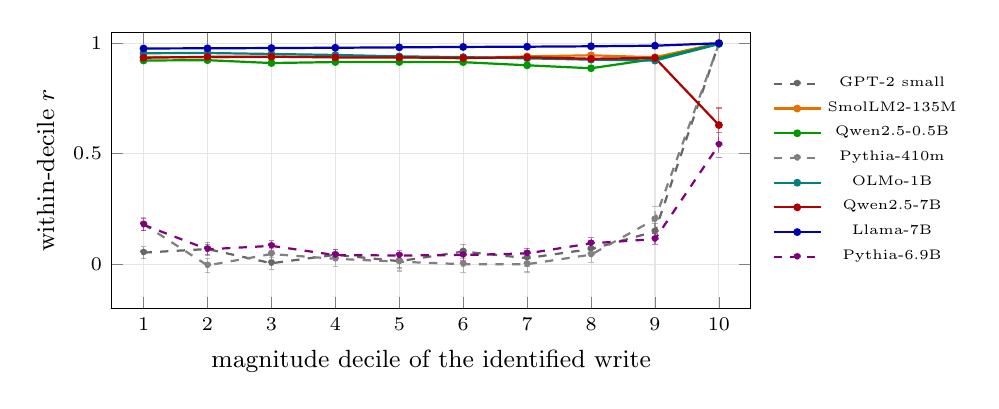
\begin{tikzpicture}\begin{axis}[width=0.8\linewidth, height=0.42\linewidth, xlabel={magnitude decile of the identified write}, ylabel={within-decile $r$}, xmin=0.5, xmax=10.5, ymin=-0.2, ymax=1.05, xtick={1,...,10}, grid=major, grid style={black!10}, legend style={font=\tiny, at={(1.02,0.5)}, anchor=west, draw=none}, tick label style={font=\scriptsize}, label style={font=\small}, error bars/y dir=both, error bars/y explicit]
\addplot[thick, dashed, color=black!60, mark=*, mark size=1pt, error bars/error bar style={opacity=0.5}] coordinates {(1,0.0528) +- (0,0.0276) (2,0.0690) +- (0,0.0305) (3,0.0048) +- (0,0.0267) (4,0.0430) +- (0,0.0248) (5,0.0142) +- (0,0.0311) (6,0.0576) +- (0,0.0325) (7,0.0280) +- (0,0.0357) (8,0.0690) +- (0,0.0301) (9,0.1484) +- (0,0.0368) (10,0.9998) +- (0,0.0000)};\addlegendentry{GPT-2 small}
\addplot[thick, color=orange!90!black, mark=*, mark size=1pt, error bars/error bar style={opacity=0.5}] coordinates {(1,0.9375) +- (0,0.0030) (2,0.9360) +- (0,0.0032) (3,0.9379) +- (0,0.0024) (4,0.9387) +- (0,0.0029) (5,0.9371) +- (0,0.0034) (6,0.9315) +- (0,0.0035) (7,0.9399) +- (0,0.0023) (8,0.9451) +- (0,0.0021) (9,0.9361) +- (0,0.0022) (10,0.9999) +- (0,0.0000)};\addlegendentry{SmolLM2-135M}
\addplot[thick, color=green!60!black, mark=*, mark size=1pt, error bars/error bar style={opacity=0.5}] coordinates {(1,0.9214) +- (0,0.0031) (2,0.9230) +- (0,0.0035) (3,0.9100) +- (0,0.0036) (4,0.9145) +- (0,0.0028) (5,0.9148) +- (0,0.0023) (6,0.9140) +- (0,0.0045) (7,0.8998) +- (0,0.0032) (8,0.8864) +- (0,0.0040) (9,0.9285) +- (0,0.0058) (10,0.9975) +- (0,0.0003)};\addlegendentry{Qwen2.5-0.5B}
\addplot[thick, dashed, color=gray, mark=*, mark size=1pt, error bars/error bar style={opacity=0.5}] coordinates {(1,0.1817) +- (0,0.0300) (2,-0.0050) +- (0,0.0328) (3,0.0464) +- (0,0.0252) (4,0.0249) +- (0,0.0346) (5,0.0118) +- (0,0.0421) (6,0.0004) +- (0,0.0356) (7,0.0005) +- (0,0.0351) (8,0.0437) +- (0,0.0340) (9,0.2037) +- (0,0.0590) (10,0.9963) +- (0,0.0005)};\addlegendentry{Pythia-410m}
\addplot[thick, color=teal, mark=*, mark size=1pt, error bars/error bar style={opacity=0.5}] coordinates {(1,0.9545) +- (0,0.0021) (2,0.9554) +- (0,0.0013) (3,0.9510) +- (0,0.0016) (4,0.9465) +- (0,0.0016) (5,0.9402) +- (0,0.0019) (6,0.9366) +- (0,0.0017) (7,0.9313) +- (0,0.0023) (8,0.9253) +- (0,0.0022) (9,0.9211) +- (0,0.0025) (10,0.9961) +- (0,0.0005)};\addlegendentry{OLMo-1B}
\addplot[thick, color=red!70!black, mark=*, mark size=1pt, error bars/error bar style={opacity=0.5}] coordinates {(1,0.9339) +- (0,0.0031) (2,0.9381) +- (0,0.0028) (3,0.9387) +- (0,0.0043) (4,0.9355) +- (0,0.0046) (5,0.9351) +- (0,0.0048) (6,0.9330) +- (0,0.0056) (7,0.9360) +- (0,0.0045) (8,0.9295) +- (0,0.0060) (9,0.9331) +- (0,0.0073) (10,0.6297) +- (0,0.0771)};\addlegendentry{Qwen2.5-7B}
\addplot[thick, color=blue!70!black, mark=*, mark size=1pt, error bars/error bar style={opacity=0.5}] coordinates {(1,0.9759) +- (0,0.0008) (2,0.9767) +- (0,0.0008) (3,0.9778) +- (0,0.0007) (4,0.9791) +- (0,0.0006) (5,0.9809) +- (0,0.0007) (6,0.9828) +- (0,0.0012) (7,0.9839) +- (0,0.0009) (8,0.9857) +- (0,0.0008) (9,0.9884) +- (0,0.0008) (10,0.9995) +- (0,0.0000)};\addlegendentry{Llama-7B}
\addplot[thick, dashed, color=violet, mark=*, mark size=1pt, error bars/error bar style={opacity=0.5}] coordinates {(1,0.1787) +- (0,0.0266) (2,0.0679) +- (0,0.0234) (3,0.0834) +- (0,0.0232) (4,0.0417) +- (0,0.0246) (5,0.0398) +- (0,0.0210) (6,0.0419) +- (0,0.0251) (7,0.0492) +- (0,0.0235) (8,0.0948) +- (0,0.0248) (9,0.1140) +- (0,0.0234) (10,0.5402) +- (0,0.0556)};\addlegendentry{Pythia-6.9B}
\end{axis}\end{tikzpicture}\caption{Within-decile correlation per model on the Pile sample, with 95\% bootstrap intervals as error bars. Solid lines are gated-MLP models, dashed non-gated.}\label{app:ci-decilefig-pile}\end{figure}
\begin{table}[H]\centering\scriptsize
\caption{The individual experiment scripts (8{,}192 states for the non-GPT-2 models, corpus-restricted embedding atoms) against the single-protocol sweep on WikiText-2 (32{,}768 states, full-vocabulary dictionaries), both over all states. Agreement within the intervals is the replication check; the remaining differences come from the token sample and the dictionary size.}\label{app:ci-old}
\begin{adjustbox}{max width=\linewidth}
\begin{tabular}{lrrrrrrrr}\toprule
Model & FVU@32, scripts & sweep & recall, scripts & sweep & $r$ id., scripts & sweep & $r$ unc., scripts & sweep \\ \midrule
GPT-2 small & 0.069 & 0.069 [0.068, 0.069] & 0.647 & 0.647 [0.637, 0.657] & 0.998 & 0.998 [0.998, 0.998] & 0.648 & 0.648 [0.648, 0.648] \\
SmolLM2-135M & 0.006 & 0.006 [0.006, 0.006] & 0.673 & 0.670 [0.661, 0.680] & 1.000 & 1.000 [1.000, 1.000] & 0.927 & 0.928 [0.927, 0.928] \\
Qwen2.5-0.5B & 0.018 & 0.017 [0.016, 0.017] & 0.458 & 0.459 [0.451, 0.467] & 0.994 & 0.994 [0.993, 0.994] & 0.556 & 0.551 [0.543, 0.559] \\
Pythia-410m & 0.051 & 0.050 [0.049, 0.051] & 0.470 & 0.481 [0.472, 0.490] & 0.978 & 0.980 [0.979, 0.981] & 0.450 & 0.452 [0.446, 0.455] \\
OLMo-1B & 0.018 & 0.019 [0.018, 0.019] & 0.703 & 0.693 [0.687, 0.699] & 0.996 & 0.997 [0.997, 0.998] & 0.971 & 0.971 [0.969, 0.972] \\
Qwen2.5-7B & 0.010 & 0.010 [0.009, 0.010] & 0.684 & 0.673 [0.663, 0.685] & 0.549 & 0.554 [0.506, 0.595] & 0.312 & 0.308 [0.271, 0.343] \\
Llama-7B & 0.088 & 0.089 [0.087, 0.090] & 0.980 & 0.981 [0.979, 0.983] & 0.999 & 0.999 [0.999, 0.999] & 0.998 & 0.998 [0.998, 0.998] \\
Pythia-6.9B & 0.309 & 0.310 [0.303, 0.315] & 0.808 & 0.787 [0.779, 0.795] & 0.522 & 0.539 [0.528, 0.551] & 0.412 & 0.424 [0.409, 0.439] \\
\bottomrule\end{tabular}\end{adjustbox}
\end{table}

\section{The Ceiling in Each Model, the Matched SAE Comparison and Sparsity at Matched Budgets}\label{app:z}
This section uses the states, dictionaries, centering and bootstrap of Appendix~\ref{app:ci}.
\subsection{Identification and survival in all models}\label{app:z3}
\texttt{exp\_z3\_ceiling} repeats the GPT-2 analysis of Table~\ref{app:survbins} and Table~\ref{app:auc} for the eight models on both corpora: each token's three dominant MLP writes (98,304 cases per model and corpus), their survival $s=(\mathbf{x}\cdot\mathbf{d})/c$ in the observed state, and whether OMP at $k=64$ places the write's atom in the support. Two further quantities decompose the misses. A miss is \emph{erased} if $s<0.25$, \emph{weakened} if $0.25\le s<0.75$, a \emph{twin} miss if the write is intact but an atom within $|\cos|\ge0.95$ of its atom sits in the support instead, and \emph{intact, unselected} otherwise. The GPT-2 row reproduces Table~\ref{app:survbins} exactly.
\begin{table}[H]\centering\scriptsize
\caption{Identification of the three dominant writes on WikiText-2 against their survival. Intact means $s\ge0.75$, erased $s<0.25$. Brackets are 95\% bootstrap intervals over sequences.}\label{app:z3-surv-wikitext}
\begin{adjustbox}{max width=\linewidth}
\begin{tabular}{lrrrrrrrr}\toprule
Model & gated & identified, all cases & share intact & identified, intact & share erased & identified, erased & AUC survival & AUC prominence \\ \midrule
GPT-2 small & no & 0.491 [0.484, 0.497] & 0.834 & 0.584 [0.577, 0.590] & 0.128 & 0.008 [0.007, 0.009] & 0.73 & 0.80 \\
SmolLM2-135M & yes & 0.494 [0.490, 0.497] & 0.761 & 0.614 [0.610, 0.618] & 0.089 & 0.015 [0.013, 0.018] & 0.81 & 0.86 \\
Qwen2.5-0.5B & yes & 0.349 [0.345, 0.353] & 0.527 & 0.550 [0.545, 0.556] & 0.104 & 0.004 [0.003, 0.006] & 0.83 & 0.92 \\
Pythia-410m & no & 0.365 [0.358, 0.371] & 0.762 & 0.465 [0.457, 0.471] & 0.080 & 0.003 [0.002, 0.004] & 0.84 & 0.91 \\
OLMo-1B & yes & 0.606 [0.602, 0.611] & 0.637 & 0.788 [0.782, 0.793] & 0.063 & 0.036 [0.030, 0.041] & 0.82 & 0.89 \\
Qwen2.5-7B & yes & 0.556 [0.547, 0.565] & 0.363 & 0.778 [0.770, 0.787] & 0.094 & 0.076 [0.067, 0.085] & 0.76 & 0.88 \\
Llama-7B & yes & 0.946 [0.944, 0.949] & 0.976 & 0.962 [0.960, 0.963] & 0.009 & 0.150 [0.122, 0.178] & 0.76 & 0.85 \\
Pythia-6.9B & no & 0.687 [0.680, 0.694] & 0.922 & 0.744 [0.737, 0.750] & 0.062 & 0.007 [0.005, 0.009] & 0.82 & 0.86 \\
\bottomrule\end{tabular}\end{adjustbox}
\end{table}
\begin{table}[H]\centering\scriptsize
\caption{Where the misses come from on WikiText-2: the share of missed dominant writes in each class (the four shares sum to one).}\label{app:z3-miss-wikitext}
\begin{adjustbox}{max width=\linewidth}
\begin{tabular}{lrrrrrr}\toprule
Model & miss rate & erased & weakened & twin in support & intact, unselected & cases with a twin in the support \\ \midrule
GPT-2 small & 0.509 & 0.25 [0.24, 0.26] & 0.07 [0.07, 0.07] & 0.00 [0.00, 0.00] & 0.68 [0.67, 0.69] & 0.2\% \\
SmolLM2-135M & 0.506 & 0.17 [0.17, 0.18] & 0.25 [0.24, 0.25] & 0.00 [0.00, 0.00] & 0.58 [0.57, 0.59] & 0.4\% \\
Qwen2.5-0.5B & 0.651 & 0.16 [0.15, 0.16] & 0.48 [0.47, 0.48] & 0.00 [0.00, 0.00] & 0.36 [0.35, 0.37] & 0.1\% \\
Pythia-410m & 0.635 & 0.13 [0.12, 0.13] & 0.23 [0.23, 0.24] & 0.01 [0.01, 0.01] & 0.64 [0.63, 0.64] & 0.3\% \\
OLMo-1B & 0.394 & 0.15 [0.15, 0.16] & 0.50 [0.49, 0.51] & 0.00 [0.00, 0.00] & 0.34 [0.33, 0.35] & 0.1\% \\
Qwen2.5-7B & 0.444 & 0.20 [0.19, 0.20] & 0.62 [0.61, 0.63] & 0.00 [0.00, 0.00] & 0.18 [0.17, 0.19] & 0.2\% \\
Llama-7B & 0.054 & 0.14 [0.12, 0.15] & 0.17 [0.16, 0.18] & 0.01 [0.01, 0.01] & 0.69 [0.67, 0.70] & 0.4\% \\
Pythia-6.9B & 0.313 & 0.20 [0.19, 0.21] & 0.05 [0.05, 0.05] & 0.00 [0.00, 0.00] & 0.75 [0.74, 0.76] & 0.0\% \\
\bottomrule\end{tabular}\end{adjustbox}
\end{table}
\begin{table}[H]\centering\scriptsize
\caption{OMP identification rate by survival bin on WikiText-2 (the six bins of Figure~\ref{fig:fvu}).}\label{app:z3-bins-wikitext}
\begin{adjustbox}{max width=\linewidth}
\begin{tabular}{lrrrrrr}\toprule
Model & $s<0$ & $[0,0.25)$ & $[0.25,0.5)$ & $[0.5,0.75)$ & $[0.75,1.25)$ & $s\ge1.25$ \\ \midrule
GPT-2 small & 0.01 & 0.01 & 0.04 & 0.11 & 0.36 & 0.62 \\
SmolLM2-135M & 0.01 & 0.04 & 0.08 & 0.22 & 0.38 & 0.71 \\
Qwen2.5-0.5B & 0.00 & 0.01 & 0.10 & 0.20 & 0.36 & 0.73 \\
Pythia-410m & 0.00 & 0.00 & 0.02 & 0.09 & 0.22 & 0.62 \\
OLMo-1B & 0.06 & 0.02 & 0.15 & 0.45 & 0.72 & 0.88 \\
Qwen2.5-7B & 0.03 & 0.08 & 0.38 & 0.60 & 0.75 & 0.85 \\
Llama-7B & 0.15 & 0.15 & 0.26 & 0.51 & 0.84 & 0.97 \\
Pythia-6.9B & 0.01 & 0.01 & 0.02 & 0.03 & 0.10 & 0.77 \\
\bottomrule\end{tabular}\end{adjustbox}
\end{table}
\begin{figure}[H]\centering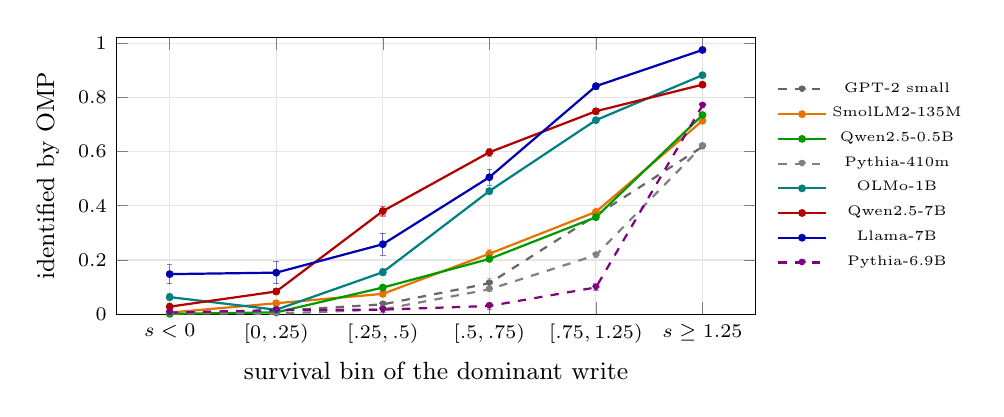
\begin{tikzpicture}\begin{axis}[width=0.8\linewidth, height=0.42\linewidth, xlabel={survival bin of the dominant write}, ylabel={identified by OMP}, xmin=0.5, xmax=6.5, ymin=0, ymax=1.02, xtick={1,...,6}, xticklabels={{$s<0$},{$[0,.25)$},{$[.25,.5)$},{$[.5,.75)$},{$[.75,1.25)$},{$s\ge1.25$}}, grid=major, grid style={black!10}, legend style={font=\tiny, at={(1.02,0.5)}, anchor=west, draw=none}, tick label style={font=\scriptsize}, label style={font=\small}, error bars/y dir=both, error bars/y explicit]
\addplot[thick, dashed, color=black!60, mark=*, mark size=1pt, error bars/error bar style={opacity=0.5}] coordinates {(1,0.0074) +- (0,0.0013) (2,0.0122) +- (0,0.0058) (3,0.0362) +- (0,0.0101) (4,0.1141) +- (0,0.0166) (5,0.3644) +- (0,0.0106) (6,0.6178) +- (0,0.0066)};\addlegendentry{GPT-2 small}
\addplot[thick, color=orange!90!black, mark=*, mark size=1pt, error bars/error bar style={opacity=0.5}] coordinates {(1,0.0058) +- (0,0.0018) (2,0.0404) +- (0,0.0087) (3,0.0750) +- (0,0.0083) (4,0.2229) +- (0,0.0152) (5,0.3774) +- (0,0.0100) (6,0.7137) +- (0,0.0057)};\addlegendentry{SmolLM2-135M}
\addplot[thick, color=green!60!black, mark=*, mark size=1pt, error bars/error bar style={opacity=0.5}] coordinates {(1,0.0012) +- (0,0.0012) (2,0.0067) +- (0,0.0025) (3,0.0982) +- (0,0.0088) (4,0.2038) +- (0,0.0088) (5,0.3578) +- (0,0.0066) (6,0.7346) +- (0,0.0074)};\addlegendentry{Qwen2.5-0.5B}
\addplot[thick, dashed, color=gray, mark=*, mark size=1pt, error bars/error bar style={opacity=0.5}] coordinates {(1,0.0039) +- (0,0.0018) (2,0.0015) +- (0,0.0015) (3,0.0179) +- (0,0.0031) (4,0.0917) +- (0,0.0062) (5,0.2178) +- (0,0.0081) (6,0.6207) +- (0,0.0097)};\addlegendentry{Pythia-410m}
\addplot[thick, color=teal, mark=*, mark size=1pt, error bars/error bar style={opacity=0.5}] coordinates {(1,0.0630) +- (0,0.0116) (2,0.0164) +- (0,0.0052) (3,0.1548) +- (0,0.0121) (4,0.4543) +- (0,0.0110) (5,0.7158) +- (0,0.0074) (6,0.8817) +- (0,0.0051)};\addlegendentry{OLMo-1B}
\addplot[thick, color=red!70!black, mark=*, mark size=1pt, error bars/error bar style={opacity=0.5}] coordinates {(1,0.0277) +- (0,0.0110) (2,0.0837) +- (0,0.0097) (3,0.3803) +- (0,0.0182) (4,0.5972) +- (0,0.0142) (5,0.7487) +- (0,0.0105) (6,0.8468) +- (0,0.0073)};\addlegendentry{Qwen2.5-7B}
\addplot[thick, color=blue!70!black, mark=*, mark size=1pt, error bars/error bar style={opacity=0.5}] coordinates {(1,0.1478) +- (0,0.0349) (2,0.1532) +- (0,0.0413) (3,0.2581) +- (0,0.0411) (4,0.5052) +- (0,0.0290) (5,0.8413) +- (0,0.0108) (6,0.9748) +- (0,0.0014)};\addlegendentry{Llama-7B}
\addplot[thick, dashed, color=violet, mark=*, mark size=1pt, error bars/error bar style={opacity=0.5}] coordinates {(1,0.0060) +- (0,0.0021) (2,0.0149) +- (0,0.0090) (3,0.0168) +- (0,0.0099) (4,0.0303) +- (0,0.0131) (5,0.0987) +- (0,0.0125) (6,0.7697) +- (0,0.0057)};\addlegendentry{Pythia-6.9B}
\end{axis}\end{tikzpicture}\caption{Identification against survival for all eight models on WikiText-2. Solid lines are gated-MLP models, dashed non-gated.}\label{app:z3-fig-wikitext}\end{figure}
\begin{table}[H]\centering\scriptsize
\caption{Identification of the three dominant writes on the Pile sample against their survival. Intact means $s\ge0.75$, erased $s<0.25$. Brackets are 95\% bootstrap intervals over sequences.}\label{app:z3-surv-pile}
\begin{adjustbox}{max width=\linewidth}
\begin{tabular}{lrrrrrrrr}\toprule
Model & gated & identified, all cases & share intact & identified, intact & share erased & identified, erased & AUC survival & AUC prominence \\ \midrule
GPT-2 small & no & 0.439 [0.423, 0.454] & 0.765 & 0.571 [0.560, 0.581] & 0.187 & 0.007 [0.005, 0.009] & 0.80 & 0.83 \\
SmolLM2-135M & yes & 0.489 [0.479, 0.497] & 0.794 & 0.594 [0.587, 0.601] & 0.082 & 0.010 [0.008, 0.012] & 0.81 & 0.88 \\
Qwen2.5-0.5B & yes & 0.365 [0.355, 0.375] & 0.573 & 0.551 [0.544, 0.559] & 0.093 & 0.002 [0.001, 0.003] & 0.84 & 0.92 \\
Pythia-410m & no & 0.346 [0.337, 0.353] & 0.735 & 0.454 [0.446, 0.461] & 0.084 & 0.004 [0.002, 0.008] & 0.83 & 0.91 \\
OLMo-1B & yes & 0.639 [0.632, 0.647] & 0.704 & 0.778 [0.771, 0.786] & 0.043 & 0.027 [0.021, 0.033] & 0.79 & 0.87 \\
Qwen2.5-7B & yes & 0.578 [0.567, 0.588] & 0.475 & 0.761 [0.750, 0.772] & 0.069 & 0.068 [0.060, 0.077] & 0.75 & 0.87 \\
Llama-7B & yes & 0.948 [0.944, 0.951] & 0.977 & 0.962 [0.960, 0.964] & 0.008 & 0.112 [0.093, 0.134] & 0.75 & 0.84 \\
Pythia-6.9B & no & 0.669 [0.656, 0.681] & 0.915 & 0.730 [0.718, 0.741] & 0.072 & 0.010 [0.007, 0.013] & 0.80 & 0.80 \\
\bottomrule\end{tabular}\end{adjustbox}
\end{table}
\begin{table}[H]\centering\scriptsize
\caption{Where the misses come from on the Pile sample: the share of missed dominant writes in each class (the four shares sum to one).}\label{app:z3-miss-pile}
\begin{adjustbox}{max width=\linewidth}
\begin{tabular}{lrrrrrr}\toprule
Model & miss rate & erased & weakened & twin in support & intact, unselected & cases with a twin in the support \\ \midrule
GPT-2 small & 0.561 & 0.33 [0.30, 0.37] & 0.08 [0.08, 0.09] & 0.00 [0.00, 0.00] & 0.58 [0.55, 0.61] & 0.3\% \\
SmolLM2-135M & 0.511 & 0.16 [0.15, 0.17] & 0.21 [0.20, 0.22] & 0.00 [0.00, 0.00] & 0.63 [0.62, 0.64] & 0.3\% \\
Qwen2.5-0.5B & 0.635 & 0.15 [0.14, 0.15] & 0.45 [0.43, 0.46] & 0.00 [0.00, 0.00] & 0.40 [0.39, 0.42] & 0.1\% \\
Pythia-410m & 0.654 & 0.13 [0.12, 0.14] & 0.26 [0.25, 0.27] & 0.01 [0.00, 0.01] & 0.61 [0.60, 0.62] & 0.3\% \\
OLMo-1B & 0.361 & 0.12 [0.11, 0.12] & 0.45 [0.44, 0.46] & 0.00 [0.00, 0.00] & 0.43 [0.41, 0.44] & 0.1\% \\
Qwen2.5-7B & 0.422 & 0.15 [0.15, 0.16] & 0.58 [0.57, 0.59] & 0.00 [0.00, 0.00] & 0.26 [0.25, 0.28] & 0.2\% \\
Llama-7B & 0.052 & 0.14 [0.13, 0.16] & 0.15 [0.14, 0.17] & 0.01 [0.01, 0.01] & 0.70 [0.67, 0.72] & 0.4\% \\
Pythia-6.9B & 0.331 & 0.22 [0.20, 0.23] & 0.04 [0.04, 0.04] & 0.00 [0.00, 0.00] & 0.74 [0.73, 0.76] & 0.1\% \\
\bottomrule\end{tabular}\end{adjustbox}
\end{table}
\begin{table}[H]\centering\scriptsize
\caption{OMP identification rate by survival bin on the Pile sample (the six bins of Figure~\ref{fig:fvu}).}\label{app:z3-bins-pile}
\begin{adjustbox}{max width=\linewidth}
\begin{tabular}{lrrrrrr}\toprule
Model & $s<0$ & $[0,0.25)$ & $[0.25,0.5)$ & $[0.5,0.75)$ & $[0.75,1.25)$ & $s\ge1.25$ \\ \midrule
GPT-2 small & 0.01 & 0.00 & 0.01 & 0.05 & 0.24 & 0.62 \\
SmolLM2-135M & 0.00 & 0.02 & 0.08 & 0.16 & 0.33 & 0.70 \\
Qwen2.5-0.5B & 0.00 & 0.00 & 0.08 & 0.20 & 0.36 & 0.74 \\
Pythia-410m & 0.00 & 0.00 & 0.01 & 0.09 & 0.23 & 0.61 \\
OLMo-1B & 0.02 & 0.03 & 0.17 & 0.45 & 0.71 & 0.86 \\
Qwen2.5-7B & 0.06 & 0.07 & 0.35 & 0.55 & 0.72 & 0.83 \\
Llama-7B & 0.08 & 0.17 & 0.37 & 0.51 & 0.81 & 0.97 \\
Pythia-6.9B & 0.01 & 0.01 & 0.03 & 0.05 & 0.11 & 0.75 \\
\bottomrule\end{tabular}\end{adjustbox}
\end{table}
\begin{figure}[H]\centering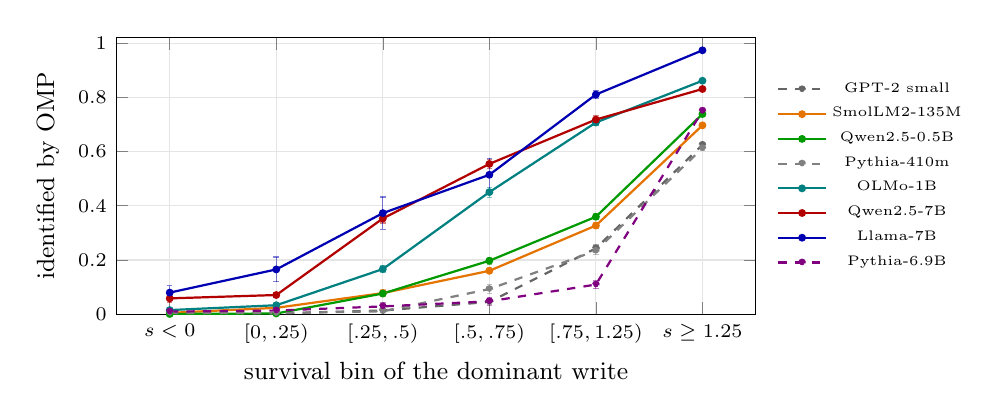
\begin{tikzpicture}\begin{axis}[width=0.8\linewidth, height=0.42\linewidth, xlabel={survival bin of the dominant write}, ylabel={identified by OMP}, xmin=0.5, xmax=6.5, ymin=0, ymax=1.02, xtick={1,...,6}, xticklabels={{$s<0$},{$[0,.25)$},{$[.25,.5)$},{$[.5,.75)$},{$[.75,1.25)$},{$s\ge1.25$}}, grid=major, grid style={black!10}, legend style={font=\tiny, at={(1.02,0.5)}, anchor=west, draw=none}, tick label style={font=\scriptsize}, label style={font=\small}, error bars/y dir=both, error bars/y explicit]
\addplot[thick, dashed, color=black!60, mark=*, mark size=1pt, error bars/error bar style={opacity=0.5}] coordinates {(1,0.0074) +- (0,0.0019) (2,0.0028) +- (0,0.0023) (3,0.0136) +- (0,0.0060) (4,0.0453) +- (0,0.0102) (5,0.2429) +- (0,0.0125) (6,0.6247) +- (0,0.0097)};\addlegendentry{GPT-2 small}
\addplot[thick, color=orange!90!black, mark=*, mark size=1pt, error bars/error bar style={opacity=0.5}] coordinates {(1,0.0048) +- (0,0.0018) (2,0.0234) +- (0,0.0072) (3,0.0778) +- (0,0.0116) (4,0.1600) +- (0,0.0111) (5,0.3270) +- (0,0.0102) (6,0.6967) +- (0,0.0071)};\addlegendentry{SmolLM2-135M}
\addplot[thick, color=green!60!black, mark=*, mark size=1pt, error bars/error bar style={opacity=0.5}] coordinates {(1,0.0008) +- (0,0.0008) (2,0.0025) +- (0,0.0014) (3,0.0762) +- (0,0.0085) (4,0.1971) +- (0,0.0128) (5,0.3594) +- (0,0.0108) (6,0.7383) +- (0,0.0077)};\addlegendentry{Qwen2.5-0.5B}
\addplot[thick, dashed, color=gray, mark=*, mark size=1pt, error bars/error bar style={opacity=0.5}] coordinates {(1,0.0048) +- (0,0.0050) (2,0.0037) +- (0,0.0026) (3,0.0107) +- (0,0.0024) (4,0.0926) +- (0,0.0157) (5,0.2339) +- (0,0.0150) (6,0.6123) +- (0,0.0085)};\addlegendentry{Pythia-410m}
\addplot[thick, color=teal, mark=*, mark size=1pt, error bars/error bar style={opacity=0.5}] coordinates {(1,0.0151) +- (0,0.0081) (2,0.0330) +- (0,0.0074) (3,0.1664) +- (0,0.0120) (4,0.4503) +- (0,0.0183) (5,0.7072) +- (0,0.0107) (6,0.8613) +- (0,0.0070)};\addlegendentry{OLMo-1B}
\addplot[thick, color=red!70!black, mark=*, mark size=1pt, error bars/error bar style={opacity=0.5}] coordinates {(1,0.0583) +- (0,0.0153) (2,0.0707) +- (0,0.0097) (3,0.3530) +- (0,0.0167) (4,0.5544) +- (0,0.0170) (5,0.7180) +- (0,0.0146) (6,0.8308) +- (0,0.0107)};\addlegendentry{Qwen2.5-7B}
\addplot[thick, color=blue!70!black, mark=*, mark size=1pt, error bars/error bar style={opacity=0.5}] coordinates {(1,0.0796) +- (0,0.0247) (2,0.1651) +- (0,0.0458) (3,0.3728) +- (0,0.0596) (4,0.5143) +- (0,0.0604) (5,0.8104) +- (0,0.0148) (6,0.9735) +- (0,0.0014)};\addlegendentry{Llama-7B}
\addplot[thick, dashed, color=violet, mark=*, mark size=1pt, error bars/error bar style={opacity=0.5}] coordinates {(1,0.0096) +- (0,0.0028) (2,0.0133) +- (0,0.0105) (3,0.0287) +- (0,0.0143) (4,0.0475) +- (0,0.0150) (5,0.1093) +- (0,0.0148) (6,0.7500) +- (0,0.0121)};\addlegendentry{Pythia-6.9B}
\end{axis}\end{tikzpicture}\caption{Identification against survival for all eight models on the Pile sample. Solid lines are gated-MLP models, dashed non-gated.}\label{app:z3-fig-pile}\end{figure}
\begin{table}[H]\centering\scriptsize
\caption{Composition of the $k=64$ support by atom type on WikiText-2.}\label{app:z3-support}
\begin{adjustbox}{max width=\linewidth}
\begin{tabular}{lrrrr}\toprule
Model & embedding & MLP & attention & bias \\ \midrule
GPT-2 small & 17.1\% & 62.1\% & 20.7\% & 0.1\% \\
SmolLM2-135M & 8.5\% & 71.4\% & 20.1\% & 0.0\% \\
Qwen2.5-0.5B & 36.4\% & 54.5\% & 9.1\% & 0.0\% \\
Pythia-410m & 32.8\% & 53.4\% & 13.8\% & 0.0\% \\
OLMo-1B & 16.1\% & 70.4\% & 13.5\% & 0.0\% \\
Qwen2.5-7B & 6.8\% & 80.5\% & 12.7\% & 0.0\% \\
Llama-7B & 2.0\% & 76.9\% & 21.1\% & 0.0\% \\
Pythia-6.9B & 3.9\% & 70.9\% & 25.2\% & 0.0\% \\
\bottomrule\end{tabular}\end{adjustbox}
\end{table}
\subsection{The SAE comparison on identical states}\label{app:z4}
\texttt{exp\_z4\_sae} evaluates the residual-stream SAEs of \citet{bloom2024} from their published weights and the weight dictionary on the same GPT-2 states in four cells: WikiText-2 with 512-token contexts (the paper's states) and OpenWebText with 128-token contexts and a leading beginning-of-text token (the SAEs' training convention), each at the state after block 5 (the input of block 6, where the SAE named \texttt{blocks.6} was trained) and after block 6 (the paper's layer, where \texttt{blocks.7} was trained). The SAEs read the residual stream in the TransformerLens frame, in which each state is centered over the model dimension, and the states are centered the same way before encoding. $L_0$ is the SAE's mean number of active features over the typical states; the weight dictionary is run at $k=32$, $k=64$ and at $k$ equal to that $L_0$. FVU is over the typical states with one denominator per cell for both methods (for GPT-2 the sink states are exactly the first positions), and $\Delta$CE is the change in next-token cross-entropy over all positions when the reconstruction replaces the state in the forward pass. On the 512-token states the SAE fails past position 127, which it never saw in training, so the two 128-token cells are the matched comparison.
\begin{table}[H]\centering\scriptsize
\caption{The trained SAE and the weight dictionary on identical GPT-2 states. Brackets are 95\% bootstrap intervals over sequences (64 WikiText-2 sequences, 256 OpenWebText documents).}\label{app:z4-table}
\begin{adjustbox}{max width=\linewidth}
\begin{tabular}{llrlrrr}\toprule
Corpus, context & state & clean CE & method & $L_0$ or $k$ & FVU, typical states & $\Delta$CE \\ \midrule
WikiText-2, 512 & after block 5 & 3.647 & SAE & 161.6 & 2.878 [2.757, 3.006] & 1.443 [1.390, 1.492] \\
 &  &  & weight dictionary & 32 & 0.325 [0.324, 0.327] & 0.521 [0.495, 0.548] \\
 &  &  & weight dictionary & 64 & 0.174 [0.173, 0.174] & 0.161 [0.150, 0.171] \\
 &  &  & weight dictionary & 162 & 0.023 [0.023, 0.023] & 0.013 [0.011, 0.015] \\
WikiText-2, 512 & after block 6 & 3.647 & SAE & 161.4 & 1.480 [1.422, 1.540] & 1.088 [1.044, 1.131] \\
 &  &  & weight dictionary & 32 & 0.338 [0.337, 0.340] & 0.551 [0.522, 0.581] \\
 &  &  & weight dictionary & 64 & 0.179 [0.179, 0.180] & 0.178 [0.167, 0.189] \\
 &  &  & weight dictionary & 161 & 0.024 [0.024, 0.024] & 0.015 [0.013, 0.017] \\
OpenWebText, 128 & after block 5 & 3.323 & SAE & 51.2 & 0.109 [0.107, 0.111] & 0.144 [0.135, 0.155] \\
 &  &  & weight dictionary & 32 & 0.307 [0.306, 0.308] & 0.428 [0.411, 0.448] \\
 &  &  & weight dictionary & 51 & 0.210 [0.209, 0.211] & 0.188 [0.179, 0.197] \\
 &  &  & weight dictionary & 64 & 0.163 [0.162, 0.164] & 0.125 [0.118, 0.132] \\
OpenWebText, 128 & after block 6 & 3.323 & SAE & 58.8 & 0.121 [0.119, 0.123] & 0.155 [0.145, 0.165] \\
 &  &  & weight dictionary & 32 & 0.320 [0.319, 0.321] & 0.477 [0.460, 0.497] \\
 &  &  & weight dictionary & 59 & 0.187 [0.186, 0.187] & 0.172 [0.165, 0.181] \\
 &  &  & weight dictionary & 64 & 0.169 [0.169, 0.170] & 0.146 [0.138, 0.154] \\
\bottomrule\end{tabular}\end{adjustbox}
\end{table}
\subsection{Sparsity at matched budgets}\label{app:z5}
\texttt{exp\_z5\_kcurve} sweeps $k$ for the weight dictionary and its rotation on 8,192 WikiText-2 states per model (the first 16 evaluation sequences of the sweep), reading the FVU at $k=4$ to $256$ and at the matched budgets $k=d/16$ and $k=d/12$, so that models of different width are compared at the same fraction of their dimension. The table and the figure are over the typical states.
\begin{table}[H]\centering\scriptsize
\caption{FVU of the typical states at a fixed budget of 32 atoms, at budgets matched to the width, and at 256 atoms.}\label{app:z5-table}
\begin{adjustbox}{max width=\linewidth}
\begin{tabular}{lrrrrrrrrrrr}\toprule
Model & $d$ & weight, $k=32$ & rotated, $k=32$ & $k=d/16$ & weight & rotated & $k=d/12$ & weight & rotated & weight, $k=256$ & rotated, $k=256$ \\ \midrule
GPT-2 small & 768 & 0.334 & 0.530 & 48 & 0.243 & 0.391 & 64 & 0.177 & 0.288 & 0.002 & 0.004 \\
SmolLM2-135M & 576 & 0.270 & 0.421 & 36 & 0.242 & 0.379 & 48 & 0.175 & 0.276 & 0.000 & 0.000 \\
Qwen2.5-0.5B & 896 & 0.407 & 0.527 & 56 & 0.255 & 0.330 & 74 & 0.180 & 0.231 & 0.003 & 0.004 \\
Pythia-410m & 1024 & 0.501 & 0.592 & 64 & 0.301 & 0.359 & 85 & 0.216 & 0.257 & 0.010 & 0.013 \\
OLMo-1B & 2048 & 0.564 & 0.773 & 128 & 0.269 & 0.382 & 170 & 0.197 & 0.280 & 0.102 & 0.145 \\
Qwen2.5-7B & 3584 & 0.543 & 0.847 & 224 & 0.210 & 0.351 & 298 & 0.150 & 0.249 & 0.182 & 0.303 \\
Llama-7B & 4096 & 0.621 & 0.872 & 256 & 0.245 & 0.380 & 341 & 0.178 & 0.277 & 0.245 & 0.380 \\
Pythia-6.9B & 4096 & 0.707 & 0.868 & 256 & 0.279 & 0.363 & 341 & 0.199 & 0.260 & 0.279 & 0.363 \\
\bottomrule\end{tabular}\end{adjustbox}
\end{table}
\begin{figure}[H]\centering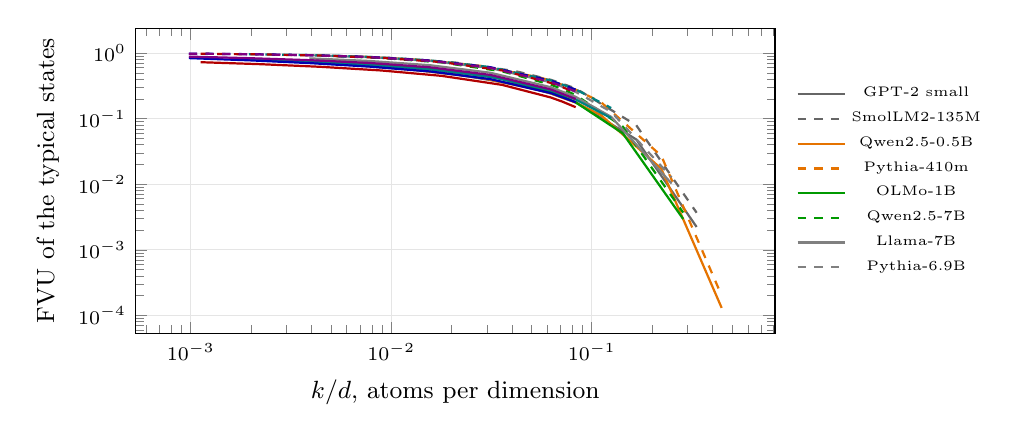
\begin{tikzpicture}\begin{axis}[width=0.8\linewidth, height=0.45\linewidth, xmode=log, ymode=log, xlabel={$k/d$, atoms per dimension}, ylabel={FVU of the typical states}, grid=major, grid style={black!10}, legend style={font=\tiny, at={(1.02,0.5)}, anchor=west, draw=none}, tick label style={font=\scriptsize}, label style={font=\small}]
\addplot[thick, color=black!60, mark=none] coordinates {(0.00521,0.70182) (0.01042,0.59594) (0.02083,0.47543) (0.04167,0.33432) (0.06250,0.24267) (0.08333,0.17722) (0.16667,0.04821) (0.33333,0.00223)};\addlegendentry{GPT-2 small}
\addplot[thick, dashed, color=black!60, mark=none] coordinates {(0.00521,0.91273) (0.01042,0.84044) (0.02083,0.71841) (0.04167,0.52985) (0.06250,0.39147) (0.08333,0.28833) (0.16667,0.07938) (0.33333,0.00368)};
\addplot[thick, color=orange!90!black, mark=none] coordinates {(0.00694,0.64552) (0.01389,0.54337) (0.02778,0.42082) (0.05556,0.26965) (0.06250,0.24208) (0.08333,0.17527) (0.11111,0.11340) (0.22222,0.01721) (0.44444,0.00013)};\addlegendentry{SmolLM2-135M}
\addplot[thick, dashed, color=orange!90!black, mark=none] coordinates {(0.00694,0.88485) (0.01389,0.79223) (0.02778,0.64034) (0.05556,0.42137) (0.06250,0.37931) (0.08333,0.27592) (0.11111,0.17888) (0.22222,0.02713) (0.44444,0.00020)};
\addplot[thick, color=green!60!black, mark=none] coordinates {(0.00446,0.76610) (0.00893,0.67655) (0.01786,0.56148) (0.03571,0.40654) (0.06250,0.25531) (0.07143,0.21853) (0.08259,0.17964) (0.14286,0.05966) (0.28571,0.00295)};\addlegendentry{Qwen2.5-0.5B}
\addplot[thick, dashed, color=green!60!black, mark=none] coordinates {(0.00446,0.91490) (0.00893,0.84295) (0.01786,0.71948) (0.03571,0.52720) (0.06250,0.33011) (0.07143,0.28188) (0.08259,0.23100) (0.14286,0.07562) (0.28571,0.00369)};
\addplot[thick, color=gray, mark=none] coordinates {(0.00391,0.83108) (0.00781,0.75796) (0.01562,0.65336) (0.03125,0.50108) (0.06250,0.30149) (0.08301,0.21573) (0.12500,0.10653) (0.25000,0.01027)};\addlegendentry{Pythia-410m}
\addplot[thick, dashed, color=gray, mark=none] coordinates {(0.00391,0.92772) (0.00781,0.86685) (0.01562,0.76126) (0.03125,0.59174) (0.06250,0.35859) (0.08301,0.25691) (0.12500,0.12712) (0.25000,0.01278)};
\addplot[thick, color=teal, mark=none] coordinates {(0.00195,0.81035) (0.00391,0.73906) (0.00781,0.65963) (0.01562,0.56372) (0.03125,0.43529) (0.06250,0.26923) (0.08301,0.19676) (0.12500,0.10192)};\addlegendentry{OLMo-1B}
\addplot[thick, dashed, color=teal, mark=none] coordinates {(0.00195,0.96293) (0.00391,0.93095) (0.00781,0.87330) (0.01562,0.77300) (0.03125,0.61051) (0.06250,0.38237) (0.08301,0.28012) (0.12500,0.14530)};
\addplot[thick, color=red!70!black, mark=none] coordinates {(0.00112,0.72614) (0.00223,0.67718) (0.00446,0.61711) (0.00893,0.54290) (0.01786,0.44912) (0.03571,0.32752) (0.06250,0.21035) (0.07143,0.18162) (0.08315,0.14961)};\addlegendentry{Qwen2.5-7B}
\addplot[thick, dashed, color=red!70!black, mark=none] coordinates {(0.00112,0.97601) (0.00223,0.95493) (0.00446,0.91628) (0.00893,0.84715) (0.01786,0.72894) (0.03571,0.54395) (0.06250,0.35087) (0.07143,0.30268) (0.08315,0.24890)};
\addplot[thick, color=blue!70!black, mark=none] coordinates {(0.00098,0.83841) (0.00195,0.77576) (0.00391,0.70340) (0.00781,0.62135) (0.01562,0.52419) (0.03125,0.40005) (0.06250,0.24508) (0.08325,0.17775)};\addlegendentry{Llama-7B}
\addplot[thick, dashed, color=blue!70!black, mark=none] coordinates {(0.00098,0.97997) (0.00195,0.96244) (0.00391,0.93023) (0.00781,0.87225) (0.01562,0.77151) (0.03125,0.60857) (0.06250,0.38024) (0.08325,0.27691)};
\addplot[thick, color=violet, mark=none] coordinates {(0.00098,0.88298) (0.00195,0.83674) (0.00391,0.77975) (0.00781,0.70718) (0.01562,0.60684) (0.03125,0.46405) (0.06250,0.27925) (0.08325,0.19927)};\addlegendentry{Pythia-6.9B}
\addplot[thick, dashed, color=violet, mark=none] coordinates {(0.00098,0.97945) (0.00195,0.96137) (0.00391,0.92807) (0.00781,0.86805) (0.01562,0.76386) (0.03125,0.59590) (0.06250,0.36345) (0.08325,0.26021)};
\end{axis}\end{tikzpicture}\caption{Reconstruction of the typical states against the relative budget $k/d$ for the weight dictionary (solid) and its rotation (dashed), eight models on WikiText-2.}\label{app:z5-fig}\end{figure}
\subsection{The GPT-2 sparsity sweep and the provenance null on typical states}\label{app:z-gpt2}
Tables~\ref{app:z-gpt2-typical} and~\ref{app:z-gpt2-all} give the GPT-2 sparsity sweep and the provenance controls of Section~\ref{sec:recon} over the typical states and over all states, from the per-token residuals of \texttt{exp\_a\_wdd} and \texttt{exp\_d\_provenance}. The sink states are 64 of the 32{,}768 layer-6 states and carry 79.7\% of the variance. The main text quotes the typical-state rows; Appendix~\ref{app:recon} has the all-state sweep with the spliced-in cross-entropies.
\begin{table}[H]\centering\scriptsize
\caption{GPT-2 layer 6, FVU against sparsity over the typical states.}\label{app:z-gpt2-typical}
\begin{adjustbox}{max width=\linewidth}
\begin{tabular}{lrrrrr}\toprule
Dictionary & $k=4$ & $k=8$ & $k=16$ & $k=32$ & $k=64$ \\ \midrule
weight dictionary & 0.707 & 0.601 & 0.481 & 0.338 & 0.179 \\
weight dictionary, no centering & 0.896 & 0.727 & 0.562 & 0.390 & 0.206 \\
sampled-activation dictionary & 0.286 & 0.222 & 0.166 & 0.113 & 0.063 \\
PCA, best $k$ per state & 0.774 & 0.684 & 0.582 & 0.469 & 0.341 \\
random directions & 0.908 & 0.832 & 0.701 & 0.500 & 0.251 \\
rotated weight dictionary & 0.912 & 0.840 & 0.718 & 0.529 & 0.288 \\
correct dictionary, subsampled to the null size & 0.723 & 0.621 & 0.502 & 0.358 & 0.194 \\
provenance null: atoms from blocks 7 to 11 & 0.810 & 0.723 & 0.608 & 0.449 & 0.252 \\
\bottomrule\end{tabular}\end{adjustbox}
\end{table}
\begin{table}[H]\centering\scriptsize
\caption{GPT-2 layer 6, FVU against sparsity over the all states.}\label{app:z-gpt2-all}
\begin{adjustbox}{max width=\linewidth}
\begin{tabular}{lrrrrr}\toprule
Dictionary & $k=4$ & $k=8$ & $k=16$ & $k=32$ & $k=64$ \\ \midrule
weight dictionary & 0.144 & 0.122 & 0.098 & 0.069 & 0.036 \\
weight dictionary, no centering & 0.182 & 0.148 & 0.114 & 0.079 & 0.042 \\
sampled-activation dictionary & 0.058 & 0.045 & 0.034 & 0.023 & 0.013 \\
PCA, best $k$ per state & 0.157 & 0.139 & 0.118 & 0.095 & 0.069 \\
random directions & 0.911 & 0.833 & 0.700 & 0.501 & 0.252 \\
rotated weight dictionary & 0.924 & 0.855 & 0.737 & 0.549 & 0.299 \\
correct dictionary, subsampled to the null size & 0.150 & 0.128 & 0.102 & 0.073 & 0.040 \\
provenance null: atoms from blocks 7 to 11 & 0.165 & 0.147 & 0.123 & 0.091 & 0.051 \\
\bottomrule\end{tabular}\end{adjustbox}
\end{table}
\subsection{What the support contains}\label{app:z6}
\texttt{exp\_z6\_selected} scores the other direction of attribution: every atom that OMP places in the $k=64$ support rather than the three dominant ledger writes. A selected MLP atom is a \emph{real} write when the ledger coefficient of its neuron at that token is at least 5\% of the token's largest write; otherwise the pursuit has spent an atom on a write that is not there. The table gives the composition of the support on the typical states, the share of selected MLP atoms that are real, the sign agreement and the median relative error of their recovered coefficients, and the share of the recovered MLP coefficient mass that sits on spurious atoms. The last columns compare OMP with a least-squares refit on the three true atoms on the same identified cases, which the main text's oracle could not do.
\begin{table}[H]\centering\scriptsize
\caption{The $k=64$ support on WikiText-2, typical states. The first three columns are the composition of the support by atom type; the next five describe the selected MLP atoms; the last four compare OMP and the true-top-3 refit on the same identified dominant writes.}\label{app:z6-wikitext}
\begin{adjustbox}{max width=\linewidth}
\begin{tabular}{lrrrrrrrrrrrr}\toprule
Model & MLP & attn. & emb. & real share of selected MLP atoms & sign & rel. error & ratio & spurious mass & $r$ OMP & $r$ refit & rel. err. OMP & rel. err. refit \\ \midrule
GPT-2 small & 62\% & 21\% & 17\% & 0.35 [0.34, 0.35] & 88.5\% & 1.55 & 2.07 & 57\% & 0.582 & 0.407 & 0.44 & 0.68 \\
SmolLM2-135M & 71\% & 20\% & 8\% & 0.24 [0.24, 0.24] & 90.4\% & 4.10 & 3.91 & 68\% & 0.835 & 0.860 & 0.54 & 0.69 \\
Qwen2.5-0.5B & 54\% & 9\% & 36\% & 0.28 [0.28, 0.28] & 92.3\% & 3.03 & 3.24 & 65\% & 0.819 & 0.838 & 0.46 & 0.47 \\
Pythia-410m & 53\% & 14\% & 33\% & 0.29 [0.29, 0.30] & 80.2\% & 3.03 & 2.34 & 67\% & 0.322 & 0.307 & 0.41 & 0.54 \\
OLMo-1B & 70\% & 14\% & 16\% & 0.51 [0.51, 0.51] & 97.0\% & 1.27 & 2.14 & 44\% & 0.907 & 0.925 & 0.34 & 0.29 \\
Qwen2.5-7B & 80\% & 13\% & 7\% & 0.43 [0.42, 0.43] & 99.0\% & 1.12 & 2.07 & 57\% & 0.887 & 0.882 & 0.50 & 0.38 \\
Llama-7B & 77\% & 21\% & 2\% & 0.71 [0.71, 0.71] & 99.1\% & 1.08 & 2.05 & 25\% & 0.982 & 0.977 & 0.25 & 0.57 \\
Pythia-6.9B & 71\% & 25\% & 4\% & 0.53 [0.53, 0.54] & 96.9\% & 2.18 & 3.07 & 41\% & 0.645 & 0.602 & 1.03 & 1.62 \\
\bottomrule\end{tabular}\end{adjustbox}
\end{table}
\begin{table}[H]\centering\scriptsize
\caption{The $k=64$ support on the Pile sample, typical states. The first three columns are the composition of the support by atom type; the next five describe the selected MLP atoms; the last four compare OMP and the true-top-3 refit on the same identified dominant writes.}\label{app:z6-pile}
\begin{adjustbox}{max width=\linewidth}
\begin{tabular}{lrrrrrrrrrrrr}\toprule
Model & MLP & attn. & emb. & real share of selected MLP atoms & sign & rel. error & ratio & spurious mass & $r$ OMP & $r$ refit & rel. err. OMP & rel. err. refit \\ \midrule
GPT-2 small & 60\% & 22\% & 17\% & 0.35 [0.35, 0.35] & 87.9\% & 1.78 & 2.20 & 57\% & 0.557 & 0.410 & 0.51 & 0.74 \\
SmolLM2-135M & 71\% & 21\% & 8\% & 0.24 [0.24, 0.25] & 89.9\% & 4.28 & 3.96 & 68\% & 0.864 & 0.883 & 0.58 & 0.72 \\
Qwen2.5-0.5B & 54\% & 10\% & 36\% & 0.28 [0.28, 0.28] & 93.2\% & 3.13 & 3.41 & 65\% & 0.830 & 0.850 & 0.44 & 0.45 \\
Pythia-410m & 53\% & 14\% & 33\% & 0.29 [0.29, 0.29] & 80.4\% & 3.13 & 2.37 & 67\% & 0.300 & 0.311 & 0.39 & 0.51 \\
OLMo-1B & 70\% & 15\% & 15\% & 0.52 [0.52, 0.52] & 97.0\% & 1.37 & 2.24 & 45\% & 0.915 & 0.930 & 0.32 & 0.28 \\
Qwen2.5-7B & 79\% & 15\% & 6\% & 0.44 [0.44, 0.44] & 98.8\% & 1.37 & 2.31 & 57\% & 0.882 & 0.875 & 0.46 & 0.36 \\
Llama-7B & 78\% & 20\% & 2\% & 0.71 [0.70, 0.71] & 99.0\% & 1.14 & 2.11 & 25\% & 0.984 & 0.971 & 0.29 & 0.62 \\
Pythia-6.9B & 72\% & 25\% & 3\% & 0.54 [0.53, 0.54] & 96.4\% & 2.27 & 3.14 & 41\% & 0.674 & 0.642 & 1.08 & 1.70 \\
\bottomrule\end{tabular}\end{adjustbox}
\end{table}
\subsection{Recall by magnitude}\label{app:recall-decile}
Top-1 recall of the largest write by decile of its magnitude, with the deciles defined over all typical-state cases before any conditioning on identification. Identification rises with the magnitude of the write in the non-gated models and in Llama-7B, and is flat or hump-shaped in the small gated models.
\begin{table}[H]\centering\scriptsize
\caption{Top-1 recall by magnitude decile of the largest write on WikiText-2.}\label{app:recall-decile-wikitext}
\begin{adjustbox}{max width=\linewidth}
\begin{tabular}{lrrrrrrrrrr}\toprule
Model & 1 & 2 & 3 & 4 & 5 & 6 & 7 & 8 & 9 & 10 \\ \midrule
GPT-2 small & 0.40 & 0.44 & 0.51 & 0.58 & 0.63 & 0.71 & 0.70 & 0.72 & 0.84 & 0.96 \\
SmolLM2-135M & 0.56 & 0.54 & 0.63 & 0.68 & 0.71 & 0.69 & 0.77 & 0.75 & 0.69 & 0.66 \\
Qwen2.5-0.5B & 0.26 & 0.39 & 0.49 & 0.56 & 0.54 & 0.44 & 0.40 & 0.42 & 0.49 & 0.61 \\
Pythia-410m & 0.35 & 0.38 & 0.35 & 0.45 & 0.45 & 0.46 & 0.53 & 0.66 & 0.66 & 0.61 \\
OLMo-1B & 0.41 & 0.52 & 0.59 & 0.65 & 0.71 & 0.74 & 0.78 & 0.83 & 0.84 & 0.85 \\
Qwen2.5-7B & 0.42 & 0.49 & 0.54 & 0.62 & 0.67 & 0.71 & 0.74 & 0.79 & 0.84 & 0.92 \\
Llama-7B & 0.90 & 0.96 & 0.98 & 0.99 & 1.00 & 1.00 & 1.00 & 1.00 & 1.00 & 1.00 \\
Pythia-6.9B & 0.60 & 0.49 & 0.53 & 0.81 & 0.83 & 0.84 & 0.86 & 0.90 & 0.92 & 0.94 \\
\bottomrule\end{tabular}\end{adjustbox}
\end{table}
\begin{table}[H]\centering\scriptsize
\caption{Top-1 recall by magnitude decile of the largest write on the Pile sample.}\label{app:recall-decile-pile}
\begin{adjustbox}{max width=\linewidth}
\begin{tabular}{lrrrrrrrrrr}\toprule
Model & 1 & 2 & 3 & 4 & 5 & 6 & 7 & 8 & 9 & 10 \\ \midrule
GPT-2 small & 0.29 & 0.36 & 0.43 & 0.51 & 0.56 & 0.60 & 0.63 & 0.69 & 0.75 & 0.86 \\
SmolLM2-135M & 0.41 & 0.53 & 0.72 & 0.60 & 0.72 & 0.75 & 0.75 & 0.76 & 0.70 & 0.68 \\
Qwen2.5-0.5B & 0.35 & 0.42 & 0.50 & 0.55 & 0.55 & 0.46 & 0.45 & 0.46 & 0.50 & 0.60 \\
Pythia-410m & 0.30 & 0.32 & 0.36 & 0.45 & 0.43 & 0.46 & 0.50 & 0.52 & 0.60 & 0.67 \\
OLMo-1B & 0.45 & 0.58 & 0.62 & 0.70 & 0.75 & 0.80 & 0.83 & 0.86 & 0.88 & 0.86 \\
Qwen2.5-7B & 0.44 & 0.51 & 0.56 & 0.63 & 0.69 & 0.71 & 0.77 & 0.82 & 0.86 & 0.93 \\
Llama-7B & 0.89 & 0.96 & 0.98 & 0.99 & 0.99 & 1.00 & 1.00 & 1.00 & 1.00 & 1.00 \\
Pythia-6.9B & 0.59 & 0.62 & 0.59 & 0.79 & 0.82 & 0.84 & 0.85 & 0.86 & 0.86 & 0.79 \\
\bottomrule\end{tabular}\end{adjustbox}
\end{table}
\subsection{The provenance null without embeddings}\label{app:d2}
\texttt{exp\_d2\_null\_noemb} repeats the provenance control of Section~\ref{sec:recon} with the embedding rows removed from both dictionaries, so that no atom of the future-block dictionary can have written to the state.
\begin{table}[H]\centering\scriptsize
\caption{GPT-2 layer 6 without embedding atoms, FVU over the typical states.}\label{app:d2-fvu_typical}
\begin{adjustbox}{max width=\linewidth}
\begin{tabular}{lrrrrrr}\toprule
Dictionary & atoms & $k=4$ & $k=8$ & $k=16$ & $k=32$ & $k=64$ \\ \midrule
correct block atoms, blocks 0 to 6 & 26,894 & 0.707 & 0.603 & 0.486 & 0.349 & 0.195 \\
correct block atoms, subsampled to the null size & 19,210 & 0.724 & 0.624 & 0.510 & 0.375 & 0.217 \\
provenance null: block atoms of blocks 7 to 11 & 19,210 & 0.816 & 0.738 & 0.635 & 0.490 & 0.297 \\
rotated correct block atoms & 26,894 & 0.919 & 0.852 & 0.739 & 0.561 & 0.324 \\
\bottomrule\end{tabular}\end{adjustbox}
\end{table}
\begin{table}[H]\centering\scriptsize
\caption{GPT-2 layer 6 without embedding atoms, FVU over the all states.}\label{app:d2-fvu_all}
\begin{adjustbox}{max width=\linewidth}
\begin{tabular}{lrrrrrr}\toprule
Dictionary & atoms & $k=4$ & $k=8$ & $k=16$ & $k=32$ & $k=64$ \\ \midrule
correct block atoms, blocks 0 to 6 & 26,894 & 0.144 & 0.123 & 0.099 & 0.071 & 0.040 \\
correct block atoms, subsampled to the null size & 19,210 & 0.147 & 0.127 & 0.104 & 0.076 & 0.044 \\
provenance null: block atoms of blocks 7 to 11 & 19,210 & 0.166 & 0.150 & 0.129 & 0.099 & 0.060 \\
rotated correct block atoms & 26,894 & 0.920 & 0.854 & 0.740 & 0.558 & 0.319 \\
\bottomrule\end{tabular}\end{adjustbox}
\end{table}
\subsection{Energy-matched ablation controls}\label{app:x5b}
\texttt{exp\_x5b\_energy} draws random sets of block-3 neurons whose summed write energy matches that of the nine strongest counter-writers to within 5\%, from all other block-3 neurons and from the other counter-writers only, and measures the cross-entropy cost of ablating each set on the states of Appendix~\ref{app:circuit}.
\begin{table}[H]\centering\scriptsize
\caption{Cross-entropy cost of ablating energy-matched random sets against the nine strongest counter-writers (clean cross-entropy 3.6291).}\label{app:x5b-table}
\begin{adjustbox}{max width=\linewidth}
\begin{tabular}{lrrr}\toprule
Ablated set & neurons & write energy & $\Delta$CE \\ \midrule
nine strongest counter-writers & 9 & 640,105 & +0.0242 \\
any block3 neuron & 466 & 631,123 & +0.0283 \\
any block3 neuron & 418 & 646,526 & +0.0235 \\
any block3 neuron & 460 & 608,784 & +0.0262 \\
other counter writers & 455 & 608,680 & +0.0317 \\
other counter writers & 431 & 608,333 & +0.0260 \\
other counter writers & 398 & 609,067 & +0.0340 \\
\bottomrule\end{tabular}\end{adjustbox}
\end{table}
\subsection{Precision control for the 7B rows}\label{app:fp32}
The 7B-class rows of Table~\ref{tab:families} were run in bfloat16. Table~\ref{app:fp32-table} gives Qwen2.5-7B, whose aggregate $r$ on identified writes is the least stable number in the table, in both precisions on the same 8{,}192 states, the first 16 evaluation sequences. Everything agrees except the top magnitude decile, where the massive-channel writes live and where the two precisions identify different members of a handful of extreme writes, which is enough to move the aggregate.
\begin{table}[H]\centering\scriptsize
\caption{Precision control: the same script in bfloat16 and in float32 on the same 8{,}192 states.}\label{app:fp32-table}
\begin{adjustbox}{max width=\linewidth}
\begin{tabular}{lrrrrrrr}\toprule
Qwen2.5-7B, WikiText-2 & FVU at $k=32$, typical & rotated & top-1 recall & $r$ identified & $r$ unconditional & deciles 1 to 9 & decile 10 \\ \midrule
bfloat16 & 0.543 & 0.847 & 0.685 & 0.548 & 0.311 & 0.926 to 0.947 & 0.679 \\
float32 & 0.544 & 0.847 & 0.683 & 0.442 & 0.232 & 0.924 to 0.947 & 0.504 \\
\bottomrule\end{tabular}\end{adjustbox}
\end{table}

